\chapter{Evaluation} \label{chapter:evaluation} 
% Accuracy of supervised learning using k-nearest neighbour classifier model targeted on fault indentification in MaFaulDa dataset. Performace of feature selection methods on very low memeber feature sets is compared to accuracies of all possible models with taht number of features
% Data logger mearuremnt abilities are validated / is checked on a standing fan. Analysis of signals from our Pump dataset. Guide in fault labeling based on characteristic bearing frequencies.W

\section{MaFaulDa in k-nearest neighbors}
% Four types of experiments: on complete feature sets calculated in time or frequency domain, every combination is enumerated/listed of subsets with same number of features, feature selection techniques are emlored to choose features faster using heuristic/metric of similiarity and then compare the result with overall best. Simulate gradual label supply in incremental learning  without recreating it from scratch.

\subsection{Complete feature sets}
% Confusion matrix
% Knn with 5 neighbours and Euclidean metric
% On original labels  and oversampled to most populous majority label testing set of 20\% from original dataset. for bearing A to see which classes are mistaken/interchanged in prediction. There is 598 observations. The label ``normal'' is not falsly attributeted to other class in either feature set. But aother classes are assigned to be normal. Most mistakes happen on predicting outer race fault which is confused with cage fault, imbalance, and less frequency with misaligment and vise vesa. Imbalance of shaft is used for generating bearing faults that is underlying natural reason on high error rate. (Fig.~\ref{fig:evaluation:all-features-confusion-matrix})

\begin{figure}[h]
    \centering
    \begin{subfigure}[b]{0.49\textwidth}
        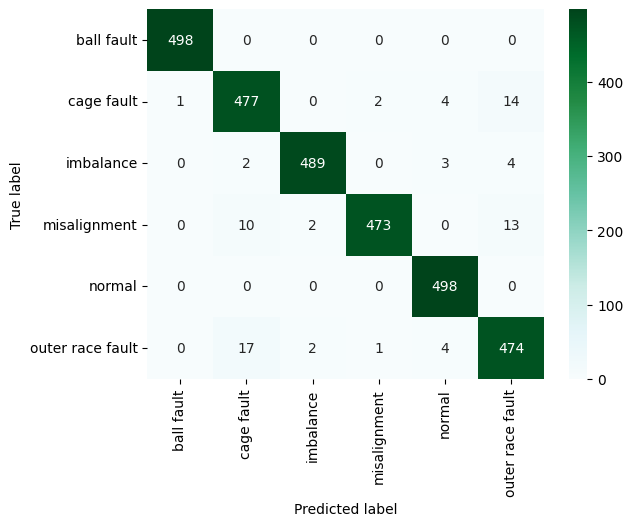
\includegraphics[width=\textwidth]{assets/results/all-features/TD-confusion-matrix.png}
        \caption{Time-domain features}
    \end{subfigure}
    \hfill
    \begin{subfigure}[b]{0.49\textwidth}
        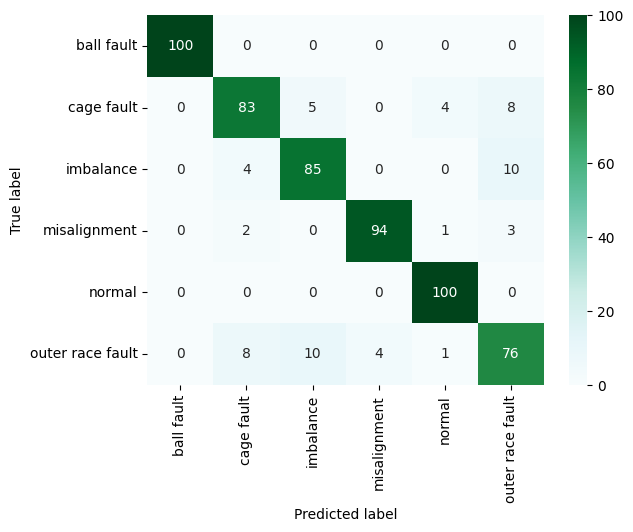
\includegraphics[width=\textwidth]{assets/results/all-features/FD-confusion-matrix.png}
        \caption{Frequency-domain features}
    \end{subfigure}
    \caption{Confusion matrix for complete sets of features}
    \label{fig:evaluation:all-features-confusion-matrix}
\end{figure}

% Nearest neighbors - how many points have neighbourhood of same class A
% e.g. we can say that less that 60\% of dataset neighbour with more than 20 taht majority of neighbouring points is in same class as the data point in question.
% This similiarity tend to favor TD feature set whose curve decreases less quickly for both labelings of MaFaulDa
\begin{figure}[h]
    \centering
    \begin{subfigure}[b]{0.49\textwidth}
        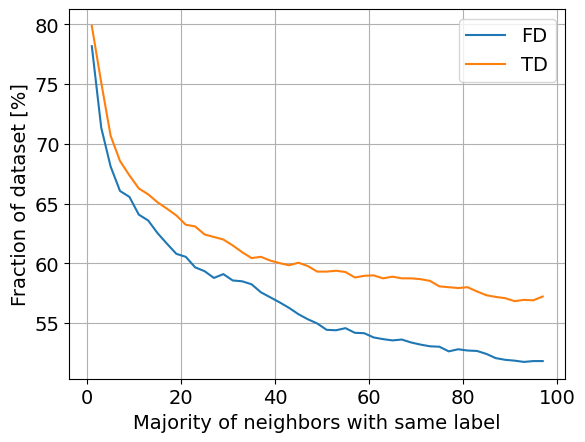
\includegraphics[width=\textwidth]{assets/results/all-features/neighborhood.png}
        \caption{No severity}
    \end{subfigure}
    \hfill
    \begin{subfigure}[b]{0.49\textwidth}
        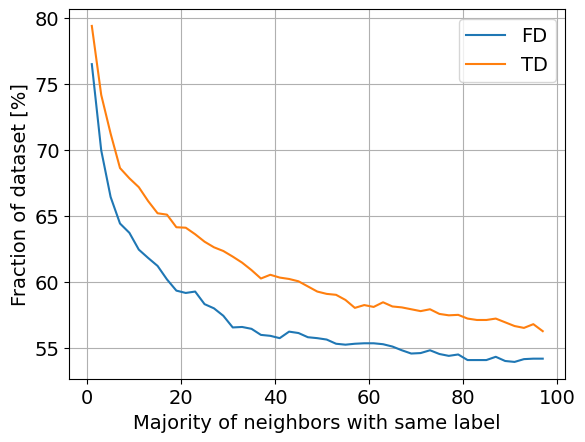
\includegraphics[width=\textwidth]{assets/results/all-features/neighborhood-severity.png}
        \caption{Severity}
    \end{subfigure}
    \caption{Neighborhood with same label}
\end{figure}

% Accuracy based on scenario - validation set in k-fold validation
% No optimal K - data is noisy - to get stable decision boundaries 
% the features creating out of all three axis reach more accurate prediction that from only the axis of motion.
% Chosen time-domain feature set is more accuracy which is observed in other experiments - probable explatations lays in large correlation among features in frequency-domain set.
% Fastest drop between 1 to 5 neighbours - sometimes 10\% decrese
\begin{figure}[h]
    \centering
    \begin{subfigure}[b]{0.48\textwidth}
        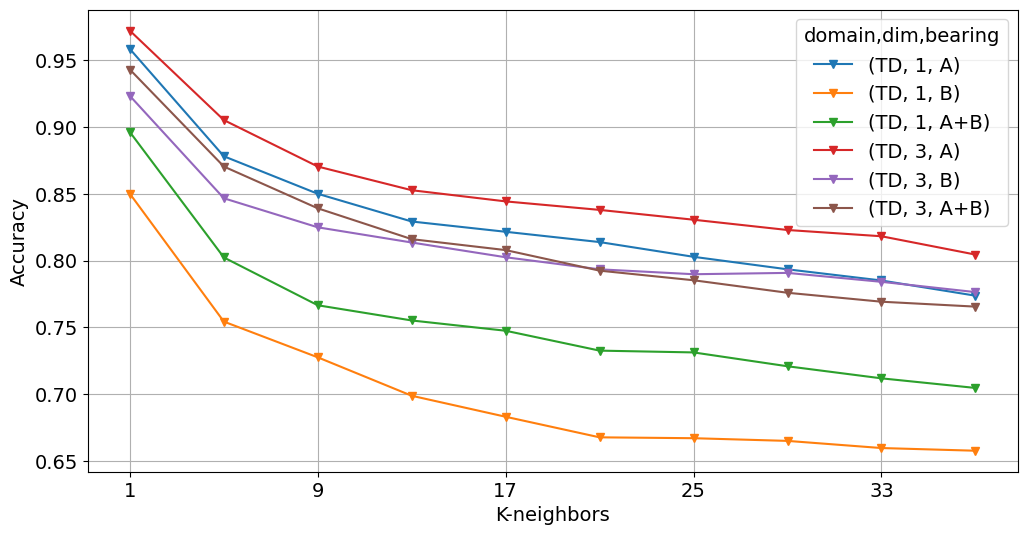
\includegraphics[width=\textwidth]{assets/results/all-features/TD.png}
        \caption{Time-domain features}
    \end{subfigure}
    \hfill
    \begin{subfigure}[b]{0.48\textwidth}
        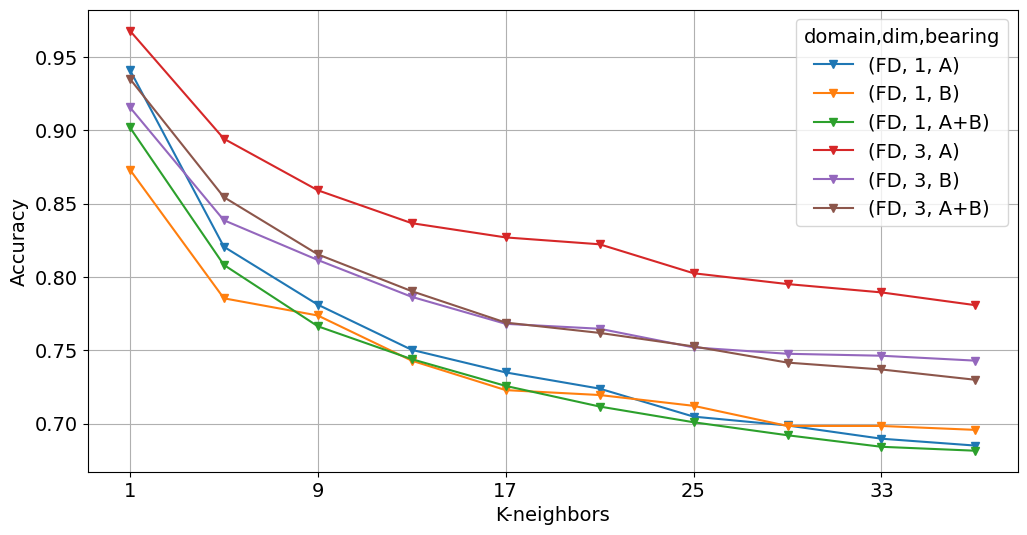
\includegraphics[width=\textwidth]{assets/results/all-features/FD.png}
        \caption{Frequency-domain features}
    \end{subfigure}
    \hfill
    \begin{subfigure}[b]{0.48\textwidth}
        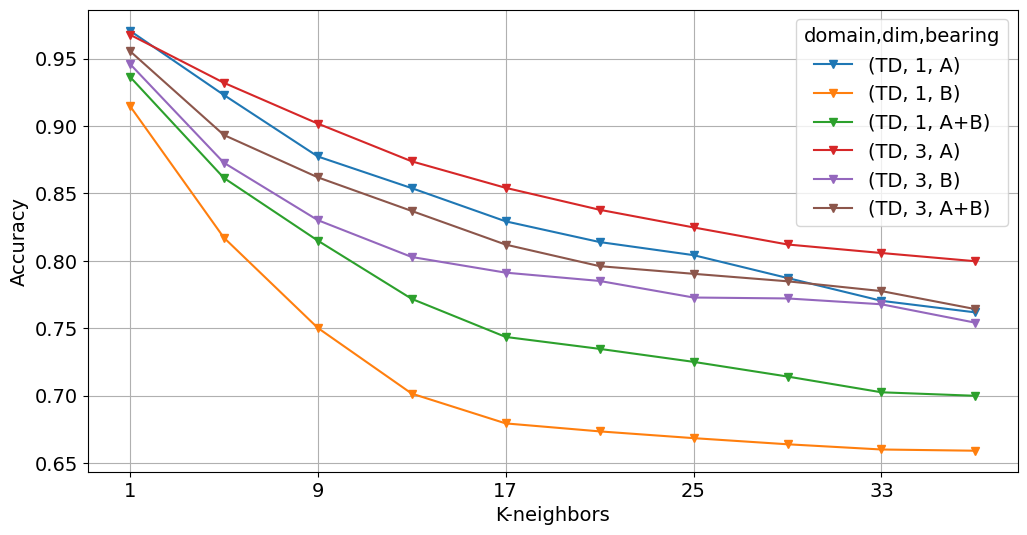
\includegraphics[width=\textwidth]{assets/results/all-features/TD-severity.png}
        \caption{Time-domain features (severity)}
    \end{subfigure}
    \hfill
    \begin{subfigure}[b]{0.48\textwidth}
        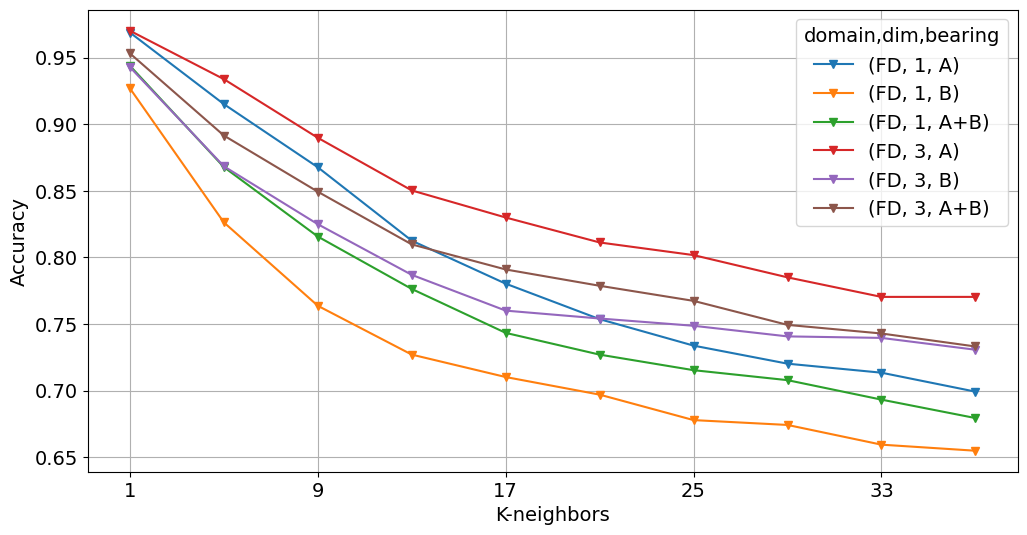
\includegraphics[width=\textwidth]{assets/results/all-features/FD-severity.png}
        \caption{Frequency-domain features (severity)}
    \end{subfigure} 
    \caption{Accuracy dependency on k-value}
\end{figure}


\subsection{Feature subset combinations}
% Boxplots
% More features - the greater accuracy - (how much) - two, three, four chosen because they can be reasonably visualized in spatial graphs or cross sections
% Compare medians of boxplots - differences

% The more neighbours less accuracy which is same as for all featues - stastically significant
% Range between IQR is between 5 - 10\% and full domain from distribution is almost 20\%

% Compare all features for bearing A to ranges of feature sets

% Std around 6%
% Maximum

% Adding from 2 to 3 features inreses maximum acheivable accuracy more than adding forth feature. It is by one more for TD than FD. It is rounded to whole numbers 6\% and 3\% and after rebaleing 3\% to 2\%. For small feature sets the FD features are tad bit better average close to 1.92\% for k = 5 but for other values of k it is not not so. The fall in accuracy by raising the number of features slows down.
% TD (no): FT: 2 (78.31), 3 (85.67), 4 (89.55)   | K: 3 (0.943316), 5 (0.917118), 11 (0.876470)
% FD (no): FT: 2 (81.52), 3 (87.52), 4 (90.26)   | K: 3 (0.940833), 5 (0.921863), 11 (0.871503)
% TD (yes): 2 (88.89), 3 (91.71), 4 (93.61)   | K: 3, 5, 11
% FD (yes): 2 (89.45), 3 (92.18), 4 (93.76)   | K: 3, 5, 11

\begin{figure}[h]
    \centering
    \begin{subfigure}[b]{0.48\textwidth}
        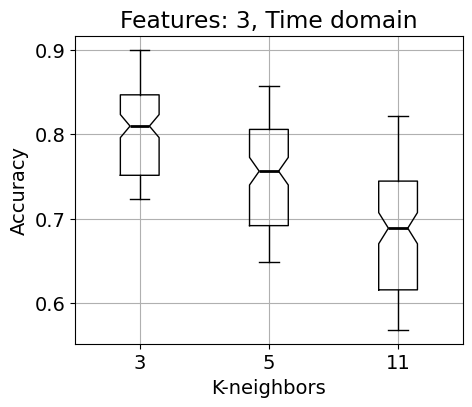
\includegraphics[width=\textwidth]{assets/results/feature-combinations/TD-3-A-False-False-F3.png}
        \caption{Time domain features}
    \end{subfigure}
    \hfill
    \begin{subfigure}[b]{0.48\textwidth}
        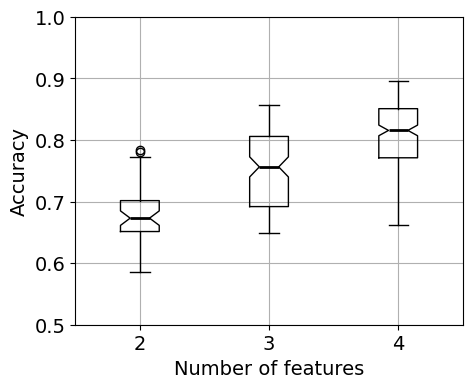
\includegraphics[width=\textwidth]{assets/results/feature-combinations/TD-3-A-False-False-K5.png}
        \caption{Time domain features}
    \end{subfigure}
    \hfill
    \begin{subfigure}[b]{0.48\textwidth}
        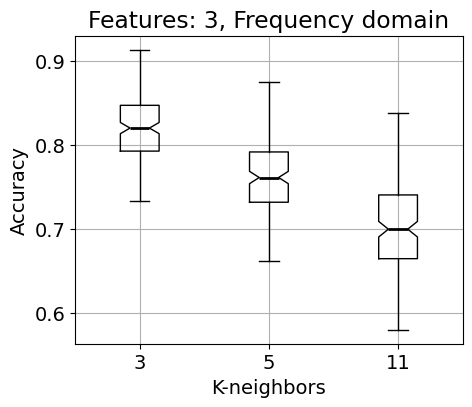
\includegraphics[width=\textwidth]{assets/results/feature-combinations/FD-3-A-False-False-F3.png}
        \caption{Frequency domain features}
    \end{subfigure}
    \hfill
    \begin{subfigure}[b]{0.48\textwidth}
        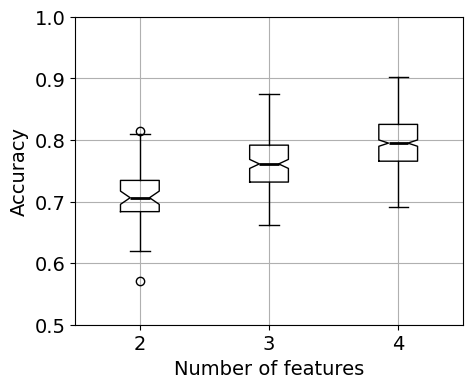
\includegraphics[width=\textwidth]{assets/results/feature-combinations/FD-3-A-False-False-K5.png}
        \caption{Frequency domain features}
    \end{subfigure}
    \caption{Model accuracy distribution (Bearings A+B, Dim = 3, Severity False)}
\end{figure}


\begin{figure}[h]
    \centering
    \begin{subfigure}[b]{0.48\textwidth}
        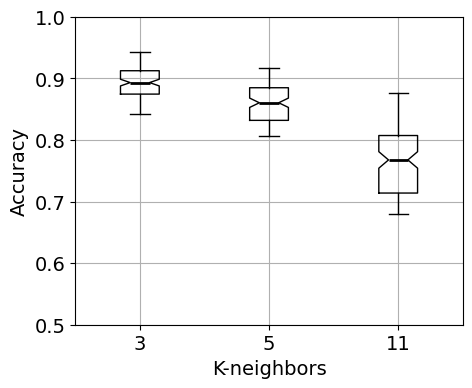
\includegraphics[width=\textwidth]{assets/results/feature-combinations/TD-3-A-True-False-F3.png}
        \caption{Time domain features}
    \end{subfigure}
    \hfill
    \begin{subfigure}[b]{0.48\textwidth}
        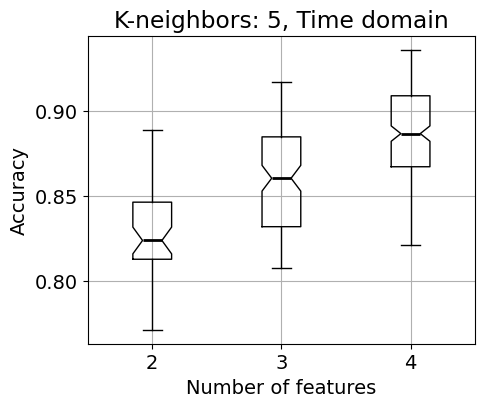
\includegraphics[width=\textwidth]{assets/results/feature-combinations/TD-3-A-True-False-K5.png}
        \caption{Time domain features}
    \end{subfigure}
    \hfill
    \begin{subfigure}[b]{0.48\textwidth}
        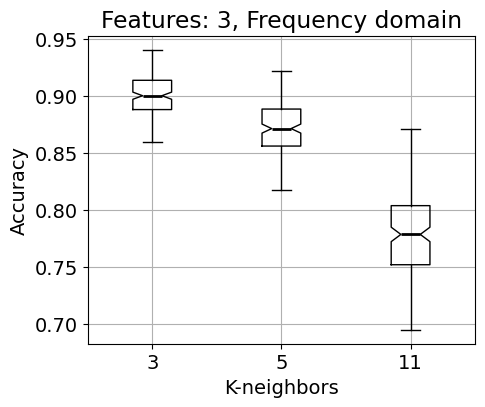
\includegraphics[width=\textwidth]{assets/results/feature-combinations/FD-3-A-True-False-F3.png}
        \caption{Frequency domain features}
    \end{subfigure}
    \hfill
    \begin{subfigure}[b]{0.48\textwidth}
        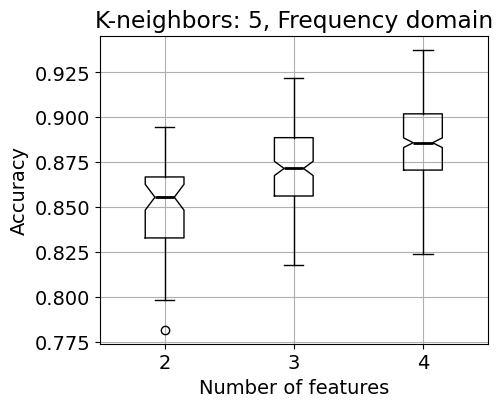
\includegraphics[width=\textwidth]{assets/results/feature-combinations/FD-3-A-True-False-K5.png}
        \caption{Frequency domain features}
    \end{subfigure}
    \caption{Model accuracy distribution (Severity True)}
\end{figure}


\subsection{Feature selection techniques}
% Accuracy tables
% Compare linear complexity accuracy with whole distribution

% Comparing test accuracy to train accuracy - large difference - the model is likely overfitting, difference is more pronounced in one axis

% In all methods the norm of three axis are better than using a single one.
% ACC set / all features / best  triplet / rank product
% Percentile

% Pecentile of best features in test is calculated against train distribution ACC: 84.07 / 99.17 in TD, ACC: 99.39 in FD. [relabel: ]
% Rank product picks 90.00 in TD (zerocross, pp, rms), 96.36 percentile of accuracies in FD (entropy, centroid, flux) [95.83 (TD) zerocross, shape, rms; 100.00 (FD) entropy, centroid, flux]
- 

% Most feature selection methods choose 
% - rank product weeds up weaker method - it get overrulled


% Furure work - more features from one recoding - in windows
% Different election methods and metrics
% Combine feature selection with 
% Find other ML model also suitable HoeffdingTreeClassifier - losing original data for labeling - mechnaism of transforming samples to model represntatin

\begin{figure}[h]
    \centering
    \begin{subfigure}[b]{0.48\textwidth}
        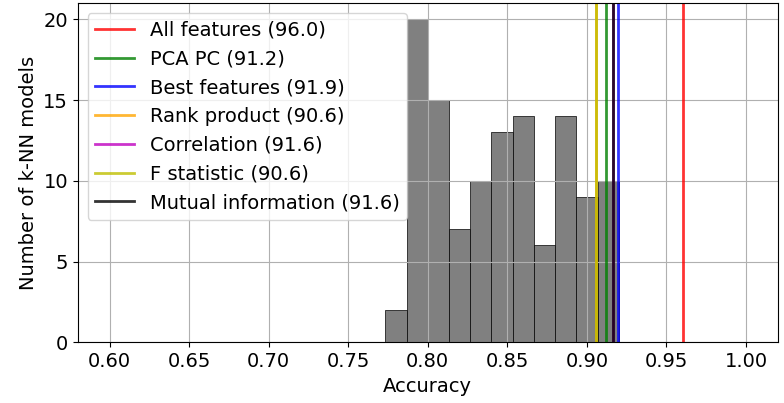
\includegraphics[width=\textwidth]{assets/results/feature-combinations/model-distr-fsel-k5-f3-TD-train.png}
        \caption{Time domain features (train)}
    \end{subfigure}
    \hfill
    \begin{subfigure}[b]{0.48\textwidth}
        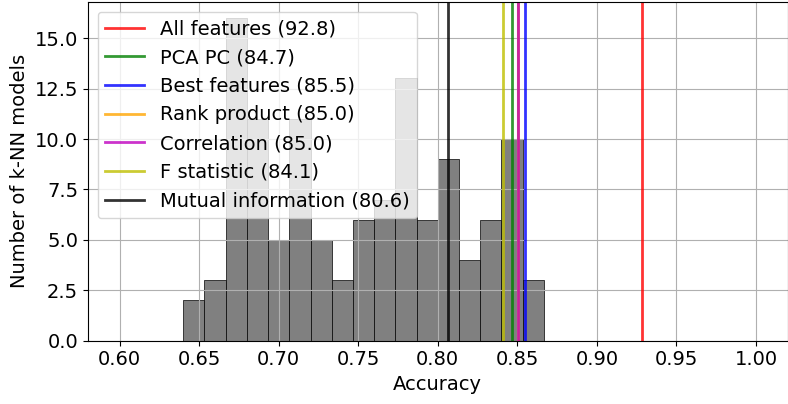
\includegraphics[width=\textwidth]{assets/results/feature-combinations/model-distr-fsel-k5-f3-TD-test.png}
        \caption{Time domain features (test)}
    \end{subfigure}
    \hfill
    \begin{subfigure}[b]{0.48\textwidth}
        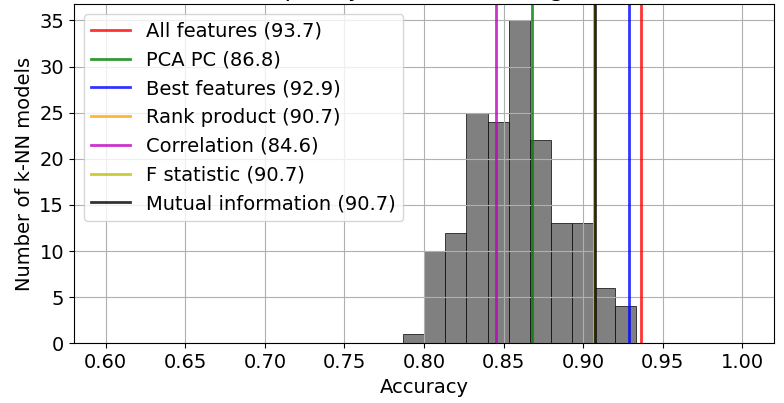
\includegraphics[width=\textwidth]{assets/results/feature-combinations/model-distr-fsel-k5-f3-FD-train.png}
        \caption{Frequency domain features (train)}
    \end{subfigure}
    \hfill
    \begin{subfigure}[b]{0.48\textwidth}
        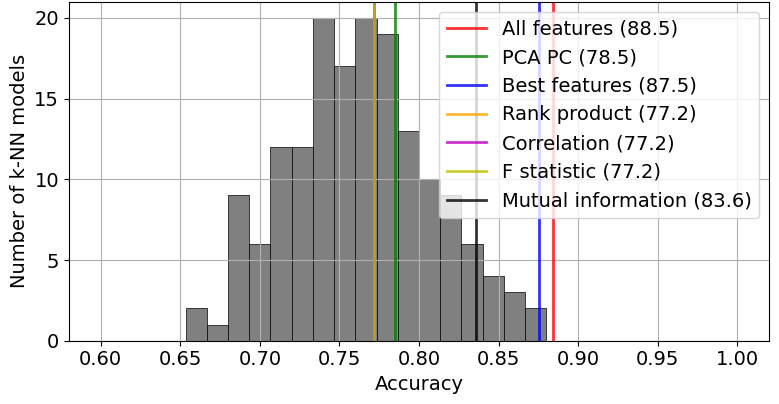
\includegraphics[width=\textwidth]{assets/results/feature-combinations/model-distr-fsel-k5-f3-FD-test.png}
        \caption{Frequency domain features (test)}
    \end{subfigure}
    \caption{Model distibution with feature selection methods (k = 5, f = 3)}
\end{figure}





\begin{table}[h]
\begin{adjustbox}{width=\textwidth}
\begin{tabular}{|l|rr|rr|r|l|}
\hline
\multirow{2}{*}{\textbf{Feature set}} & \multicolumn{2}{l|}{\textbf{Accuracy}}                                   & \multicolumn{2}{l|}{\textbf{Percentile}}                 & \multicolumn{1}{l|}{\multirow{2}{*}{\textbf{Axis}}} & \multirow{2}{*}{\textbf{Best features}} \\ \cline{2-5}
                                      & \multicolumn{1}{l|}{\textbf{Train}} & \multicolumn{1}{l|}{\textbf{Test}} & \multicolumn{1}{l|}{\textbf{Train}} & \multicolumn{1}{l|}{\textbf{Test}} & \multicolumn{1}{l|}{}                               &                                         \\ \hline
All features                          & \multicolumn{1}{r|}{92.52}          & 87.68                              & \multicolumn{1}{r|}{100.00}         & 100.00                             & 1                                                   &                                         \\ \hline
PCA PC                                & \multicolumn{1}{r|}{87.90}          & 79.42                              & \multicolumn{1}{r|}{96.67}          & 96.67                              & 1                                                   &                                         \\ \hline
Best features                         & \multicolumn{1}{r|}{89.70}          & 81.96                              & \multicolumn{1}{r|}{100.00}         & 100.00                             & 1                                                   & zerocross, pp, skewness                 \\ \hline
Rank product                          & \multicolumn{1}{r|}{87.51}          & 79.35                              & \multicolumn{1}{r|}{95.83}          & 96.67                              & 1                                                   & zerocross, shape, pp                    \\ \hline
Correlation                           & \multicolumn{1}{r|}{87.51}          & 79.35                              & \multicolumn{1}{r|}{95.83}          & 96.67                              & 1                                                   & shape, zerocross, pp                    \\ \hline
F statistic                           & \multicolumn{1}{r|}{87.51}          & 79.35                              & \multicolumn{1}{r|}{95.83}          & 96.67                              & 1                                                   & pp, zerocross, shape                    \\ \hline
Mutual information                    & \multicolumn{1}{r|}{86.98}          & 78.28                              & \multicolumn{1}{r|}{89.17}          & 94.17                              & 1                                                   & zerocross, shape, rms                   \\ \hline
All features                          & \multicolumn{1}{r|}{96.03}          & 92.80                              & \multicolumn{1}{r|}{100.00}         & 100.00                             & 3                                                   &                                         \\ \hline
PCA PC                                & \multicolumn{1}{r|}{91.20}          & 84.67                              & \multicolumn{1}{r|}{95.00}          & 93.33                              & 3                                                   &                                         \\ \hline
Best features                         & \multicolumn{1}{r|}{91.93}          & 85.47                              & \multicolumn{1}{r|}{100.00}         & 99.17                              & 3                                                   & zerocross, pp, skewness                 \\ \hline
Rank product                          & \multicolumn{1}{r|}{91.21}          & 85.04                              & \multicolumn{1}{r|}{95.83}          & 97.50                              & 3                                                   & zerocross, shape, rms                   \\ \hline
Correlation                           & \multicolumn{1}{r|}{91.21}          & 85.04                              & \multicolumn{1}{r|}{95.83}          & 97.50                              & 3                                                   & shape, zerocross, rms                   \\ \hline
F statistic                           & \multicolumn{1}{r|}{90.59}          & 84.07                              & \multicolumn{1}{r|}{91.67}          & 90.00                              & 3                                                   & rms, pp, zerocross                      \\ \hline
Mutual information                    & \multicolumn{1}{r|}{88.24}          & 80.62                              & \multicolumn{1}{r|}{75.83}          & 76.67                              & 3                                                   & zerocross, shape, crest                 \\ \hline
\end{tabular}
\end{adjustbox}
\caption{k=5, f=3, bearing=A, severity=False, domain=TD}
\end{table}





\begin{table}[h]
\begin{adjustbox}{width=\textwidth}
\begin{tabular}{|l|rr|rr|r|l|}
\hline
\multirow{2}{*}{\textbf{Feature set}} & \multicolumn{2}{l|}{\textbf{Accuracy}}                                   & \multicolumn{2}{l|}{\textbf{Percentile}}                 & \multicolumn{1}{l|}{\multirow{2}{*}{\textbf{Axis}}} & \multirow{2}{*}{\textbf{Best features}} \\ \cline{2-5}
                                      & \multicolumn{1}{l|}{\textbf{Train}} & \multicolumn{1}{l|}{\textbf{Test}} & \multicolumn{1}{l|}{\textbf{Train}} & \multicolumn{1}{l|}{\textbf{Test}} & \multicolumn{1}{l|}{}                               &                                         \\ \hline
All features                          & \multicolumn{1}{r|}{88.15}          & 79.99                              & \multicolumn{1}{r|}{99.39}          & 98.18                              & 1                                                   &                                         \\ \hline
PCA PC                                & \multicolumn{1}{r|}{83.83}          & 74.43                              & \multicolumn{1}{r|}{77.58}          & 83.03                              & 1                                                   &                                         \\ \hline
Best features                         & \multicolumn{1}{r|}{88.93}          & 81.86                              & \multicolumn{1}{r|}{100.00}         & 100.00                             & 1                                                   & centroid, roll\_off, flux               \\ \hline
Rank product                          & \multicolumn{1}{r|}{86.87}          & 77.51                              & \multicolumn{1}{r|}{95.76}          & 93.33                              & 1                                                   & roll\_off, entropy, flux                \\ \hline
Correlation                           & \multicolumn{1}{r|}{80.54}          & 68.01                              & \multicolumn{1}{r|}{33.33}          & 31.52                              & 1                                                   & roll\_off, skewness, kurtosis           \\ \hline
F statistic                           & \multicolumn{1}{r|}{86.87}          & 77.51                              & \multicolumn{1}{r|}{95.76}          & 93.33                              & 1                                                   & roll\_off, entropy, flux                \\ \hline
Mutual information                    & \multicolumn{1}{r|}{88.11}          & 80.96                              & \multicolumn{1}{r|}{99.39}          & 99.39                              & 1                                                   & roll\_off, entropy, centroid            \\ \hline
All features                          & \multicolumn{1}{r|}{93.67}          & 88.45                              & \multicolumn{1}{r|}{100.00}         & 100.00                             & 3                                                   &                                         \\ \hline
PCA PC                                & \multicolumn{1}{r|}{86.76}          & 78.51                              & \multicolumn{1}{r|}{64.85}          & 70.91                              & 3                                                   &                                         \\ \hline
Best features                         & \multicolumn{1}{r|}{92.86}          & 87.52                              & \multicolumn{1}{r|}{100.00}         & 100.00                             & 3                                                   & centroid, roll\_off, entropy            \\ \hline
Rank product                          & \multicolumn{1}{r|}{85.79}          & 77.18                              & \multicolumn{1}{r|}{51.52}          & 57.58                              & 3                                                   & roll\_off, flux, skewness               \\ \hline
Correlation                           & \multicolumn{1}{r|}{85.79}          & 77.18                              & \multicolumn{1}{r|}{51.52}          & 57.58                              & 3                                                   & roll\_off, skewness, flux               \\ \hline
F statistic                           & \multicolumn{1}{r|}{85.79}          & 77.18                              & \multicolumn{1}{r|}{51.52}          & 57.58                              & 3                                                   & roll\_off, flux, skewness               \\ \hline
Mutual information                    & \multicolumn{1}{r|}{90.73}          & 83.60                              & \multicolumn{1}{r|}{94.55}          & 94.55                              & 3                                                   & roll\_off, entropy, noisiness           \\ \hline
\end{tabular}
\end{adjustbox}
\caption{k=5, f=3, bearing=A, severity=False, domain=FD}
\end{table}



\begin{table}[h]
\begin{adjustbox}{width=\textwidth}
\begin{tabular}{|l|rr|rr|r|l|}
\hline
\multirow{2}{*}{\textbf{Feature set}} & \multicolumn{2}{l|}{\textbf{Accuracy}}                                   & \multicolumn{2}{l|}{\textbf{Percentile}}                 & \multicolumn{1}{l|}{\multirow{2}{*}{\textbf{Axis}}} & \multirow{2}{*}{\textbf{Best features}} \\ \cline{2-5}
                                      & \multicolumn{1}{l|}{\textbf{Train}} & \multicolumn{1}{l|}{\textbf{Test}} & \multicolumn{1}{l|}{\textbf{Train}} & \multicolumn{1}{l|}{\textbf{Test}} & \multicolumn{1}{l|}{}                               &                                         \\ \hline
All features                          & \multicolumn{1}{r|}{94.99}          & 92.07                              & \multicolumn{1}{r|}{100.00}         & 100.00                             & 1                                                   &                                         \\ \hline
PCA PC                                & \multicolumn{1}{r|}{92.67}          & 89.20                              & \multicolumn{1}{r|}{84.17}          & 87.50                              & 1                                                   &                                         \\ \hline
Best features                         & \multicolumn{1}{r|}{93.99}          & 91.31                              & \multicolumn{1}{r|}{100.00}         & 100.00                             & 1                                                   & zerocross, aac, kurtosis                \\ \hline
Rank product                          & \multicolumn{1}{r|}{92.71}          & 88.55                              & \multicolumn{1}{r|}{85.00}          & 80.83                              & 1                                                   & zerocross, shape, rms                   \\ \hline
Correlation                           & \multicolumn{1}{r|}{92.71}          & 88.55                              & \multicolumn{1}{r|}{85.00}          & 80.83                              & 1                                                   & zerocross, shape, rms                   \\ \hline
F statistic                           & \multicolumn{1}{r|}{92.71}          & 88.55                              & \multicolumn{1}{r|}{85.00}          & 80.83                              & 1                                                   & zerocross, shape, rms                   \\ \hline
Mutual information                    & \multicolumn{1}{r|}{92.71}          & 88.55                              & \multicolumn{1}{r|}{85.00}          & 80.83                              & 1                                                   & zerocross, shape, rms                   \\ \hline
All features                          & \multicolumn{1}{r|}{96.42}          & 94.76                              & \multicolumn{1}{r|}{100.00}         & 100.00                             & 3                                                   &                                         \\ \hline
PCA PC                                & \multicolumn{1}{r|}{94.63}          & 92.07                              & \multicolumn{1}{r|}{100.00}         & 100.00                             & 3                                                   &                                         \\ \hline
Best features                         & \multicolumn{1}{r|}{94.58}          & 91.71                              & \multicolumn{1}{r|}{100.00}         & 99.17                              & 3                                                   & zerocross, aac, shape                   \\ \hline
Rank product                          & \multicolumn{1}{r|}{94.31}          & 91.40                              & \multicolumn{1}{r|}{98.33}          & 95.83                              & 3                                                   & zerocross, shape, rms                   \\ \hline
Correlation                           & \multicolumn{1}{r|}{94.31}          & 91.40                              & \multicolumn{1}{r|}{98.33}          & 95.83                              & 3                                                   & zerocross, shape, rms                   \\ \hline
F statistic                           & \multicolumn{1}{r|}{94.31}          & 91.40                              & \multicolumn{1}{r|}{98.33}          & 95.83                              & 3                                                   & shape, zerocross, rms                   \\ \hline
Mutual information                    & \multicolumn{1}{r|}{91.90}          & 88.51                              & \multicolumn{1}{r|}{72.50}          & 76.67                              & 3                                                   & zerocross, shape, clearance             \\ \hline
\end{tabular}
\end{adjustbox}
\caption{k=5, f=3, bearing=A, severity=True, domain=TD}
\end{table}



\begin{table}[h]
\begin{adjustbox}{width=\textwidth}
\begin{tabular}{|l|rr|rr|r|l|}
\hline
\multirow{2}{*}{\textbf{Feature set}} & \multicolumn{2}{l|}{\textbf{Accuracy}}                                   & \multicolumn{2}{l|}{\textbf{Percentile}}                 & \multicolumn{1}{l|}{\multirow{2}{*}{\textbf{Axis}}} & \multirow{2}{*}{\textbf{Best features}} \\ \cline{2-5}
                                      & \multicolumn{1}{l|}{\textbf{Train}} & \multicolumn{1}{l|}{\textbf{Test}} & \multicolumn{1}{l|}{\textbf{Train}} & \multicolumn{1}{l|}{\textbf{Test}} & \multicolumn{1}{l|}{}                               &                                         \\ \hline
All features                          & \multicolumn{1}{r|}{94.17}          & 90.94                              & \multicolumn{1}{r|}{100.00}         & 99.39                              & 1                                                   &                                         \\ \hline
PCA PC                                & \multicolumn{1}{r|}{91.49}          & 87.78                              & \multicolumn{1}{r|}{80.00}          & 86.67                              & 1                                                   &                                         \\ \hline
Best features                         & \multicolumn{1}{r|}{94.13}          & 91.37                              & \multicolumn{1}{r|}{100.00}         & 100.00                             & 1                                                   & centroid, roll\_off, flux               \\ \hline
Rank product                          & \multicolumn{1}{r|}{93.75}          & 90.29                              & \multicolumn{1}{r|}{99.39}          & 99.39                              & 1                                                   & entropy, centroid, flux                 \\ \hline
Correlation                           & \multicolumn{1}{r|}{93.75}          & 90.29                              & \multicolumn{1}{r|}{99.39}          & 99.39                              & 1                                                   & entropy, flux, centroid                 \\ \hline
F statistic                           & \multicolumn{1}{r|}{93.75}          & 90.29                              & \multicolumn{1}{r|}{99.39}          & 99.39                              & 1                                                   & entropy, flux, centroid                 \\ \hline
Mutual information                    & \multicolumn{1}{r|}{93.75}          & 90.29                              & \multicolumn{1}{r|}{99.39}          & 99.39                              & 1                                                   & centroid, entropy, flux                 \\ \hline
All features                          & \multicolumn{1}{r|}{95.20}          & 93.20                              & \multicolumn{1}{r|}{100.00}         & 100.00                             & 3                                                   &                                         \\ \hline
PCA PC                                & \multicolumn{1}{r|}{92.14}          & 88.84                              & \multicolumn{1}{r|}{69.09}          & 73.94                              & 3                                                   &                                         \\ \hline
Best features                         & \multicolumn{1}{r|}{94.64}          & 91.94                              & \multicolumn{1}{r|}{100.00}         & 99.39                              & 3                                                   & centroid, roll\_off, entropy            \\ \hline
Rank product                          & \multicolumn{1}{r|}{93.89}          & 91.24                              & \multicolumn{1}{r|}{95.15}          & 97.58                              & 3                                                   & entropy, noisiness, centroid            \\ \hline
Correlation                           & \multicolumn{1}{r|}{94.50}          & 92.19                              & \multicolumn{1}{r|}{99.39}          & 100.00                             & 3                                                   & entropy, centroid, flux                 \\ \hline
F statistic                           & \multicolumn{1}{r|}{94.50}          & 92.19                              & \multicolumn{1}{r|}{99.39}          & 100.00                             & 3                                                   & entropy, flux, centroid                 \\ \hline
Mutual information                    & \multicolumn{1}{r|}{93.32}          & 90.67                              & \multicolumn{1}{r|}{90.91}          & 91.52                              & 3                                                   & noisiness, roll\_off, entropy           \\ \hline
\end{tabular}
\end{adjustbox}
\caption{k=5, f=3, bearing=A, severity=True, domain=FD}
\end{table}






% compare percentiles
% Feature combinations accuracy
\begin{figure}[h]
    \centering
    \begin{subfigure}[b]{0.48\textwidth}
        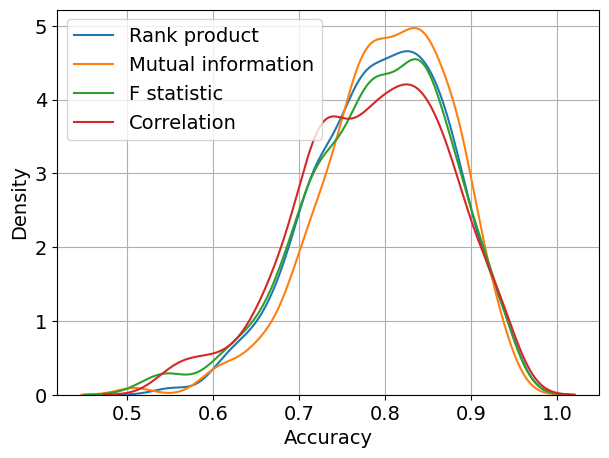
\includegraphics[width=\textwidth]{assets/results/feature-combinations/fsel-accuracy.png}
        \caption{Accuracy}
    \end{subfigure}
    \hfill
    \begin{subfigure}[b]{0.48\textwidth}
        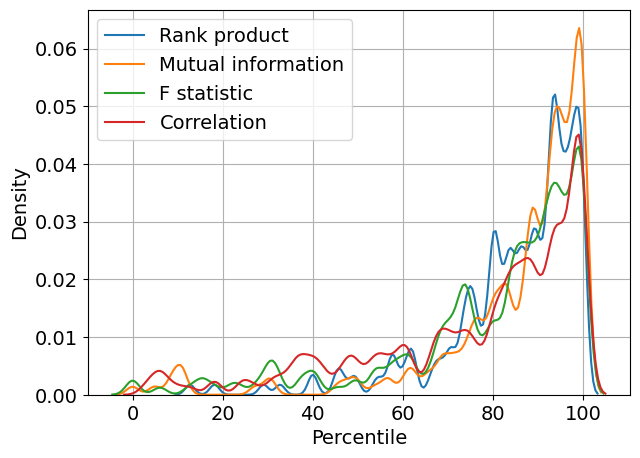
\includegraphics[width=\textwidth]{assets/results/feature-combinations/fsel-percentile.png}
        \caption{Percentile}
    \end{subfigure}
    \caption{Feature selection method choices}
\end{figure}

% In fsel percentile - mention median from notebook for each method - table
\begin{table}[h]
\centering
\begin{tabular}{|l|r|r|}
\hline
\textbf{Method}    & \multicolumn{1}{l|}{\textbf{Median percentile {[}\%{]}}} & \multicolumn{1}{l|}{\textbf{Median accuracy {[}\%{]}}} \\ \hline
Rank product       & 88.97                                                    & 79.82                                                 \\ \hline
Mutual information & 91.81                                                    & 80.87                                                 \\ \hline
F statistic        & 86.90                                                    & 79.63                                                 \\ \hline
Correlation        & 84.49                                                    & 79.04                                                  \\ \hline
\end{tabular}
\end{table}

% Best feature selection methods table (order by best count)
\begin{table}[h]
\centering
\begin{tabular}{|l|r|r|r|}
\hline
                            & \multicolumn{1}{l|}{\textbf{Best in scenarios}} & \multicolumn{1}{l|}{\textbf{Scenarios {[}\%{]}}} & \multicolumn{1}{l|}{\textbf{Mean percentile {[}\%{]}}} \\ \hline
\textbf{Rank product}       & 94                                                     & 43.52                                            & 92.38 \\ \hline
\textbf{Mutual information} & 87                                                      & 40.28                                            & 91.79 \\ \hline
\textbf{Correlation}        & 26                                                      & 12.04                                             & 97.54 \\ \hline
\textbf{F statistic}        & 9                                                       & 4.16                                             & 96.10 \\ \hline
\textbf{$\Sigma$}           & 216                                                     & 100                                       & -                                                      \\ \hline
\end{tabular}
\end{table}

% 2d and 3d plots of best features
\begin{figure}[ht]
    \centering
    \begin{subfigure}[b]{0.48\textwidth}
        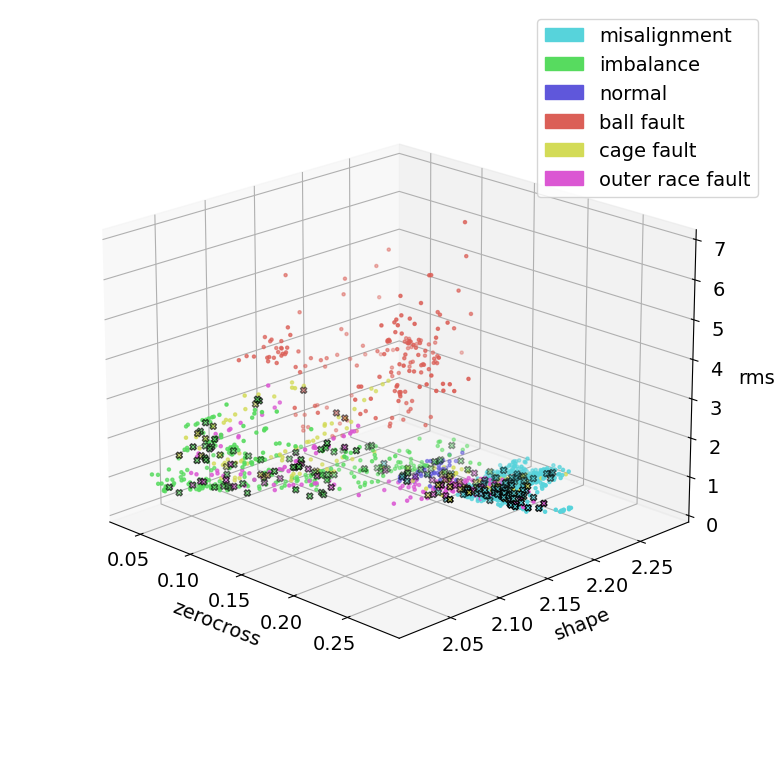
\includegraphics[width=\textwidth]{assets/results/labels/TD.png}
        \caption{Time-domain features}
    \end{subfigure}
    \hfill
    \begin{subfigure}[b]{0.48\textwidth}
        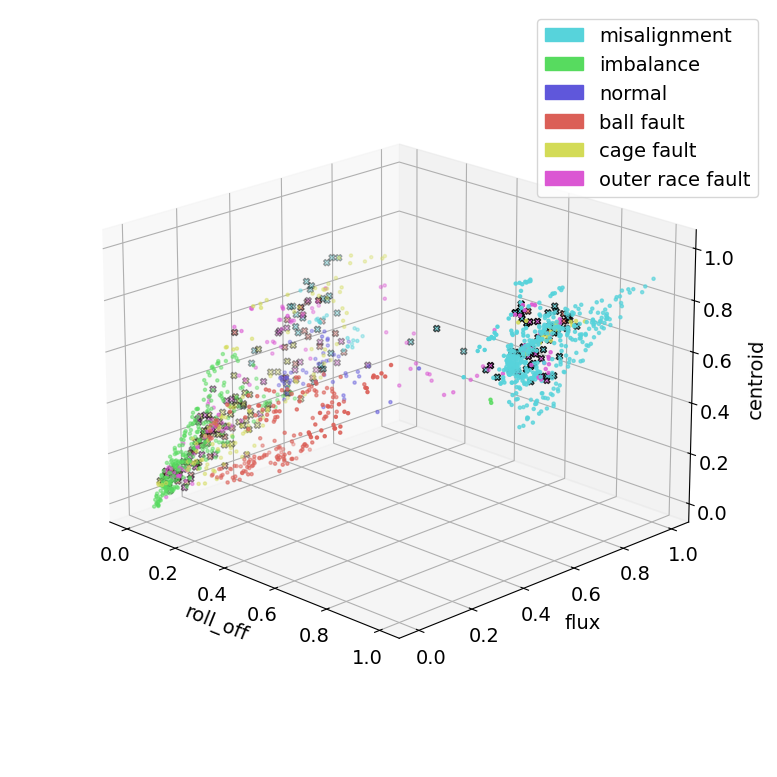
\includegraphics[width=\textwidth]{assets/results/labels/FD.png}
        \caption{Frequency-domain features}
    \end{subfigure}
    \hfill
    \begin{subfigure}[b]{0.48\textwidth}
        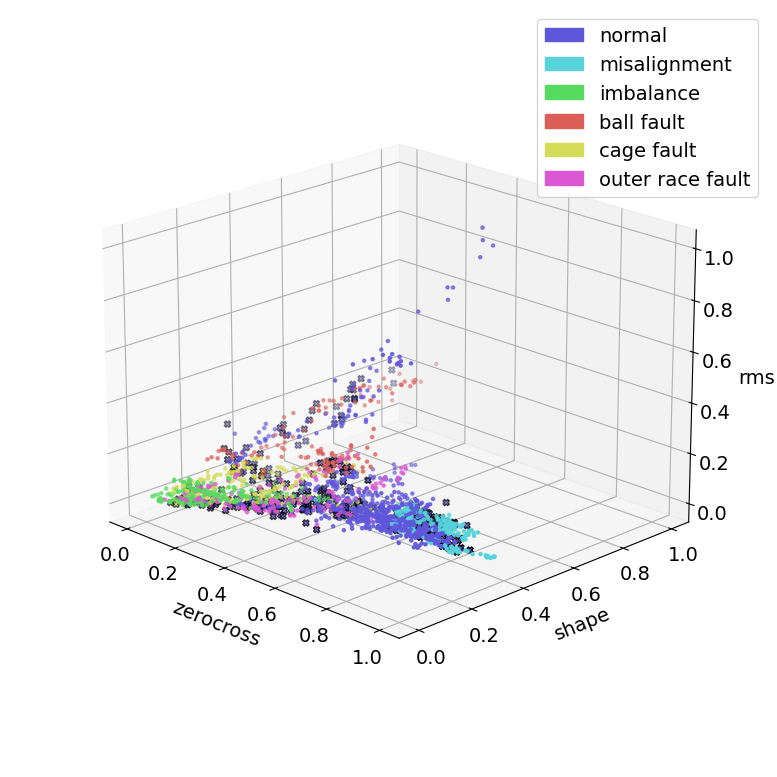
\includegraphics[width=\textwidth]{assets/results/labels/TD-severity.png}
        \caption{Time-domain features (severity)}
    \end{subfigure}
    \hfill
    \begin{subfigure}[b]{0.48\textwidth}
        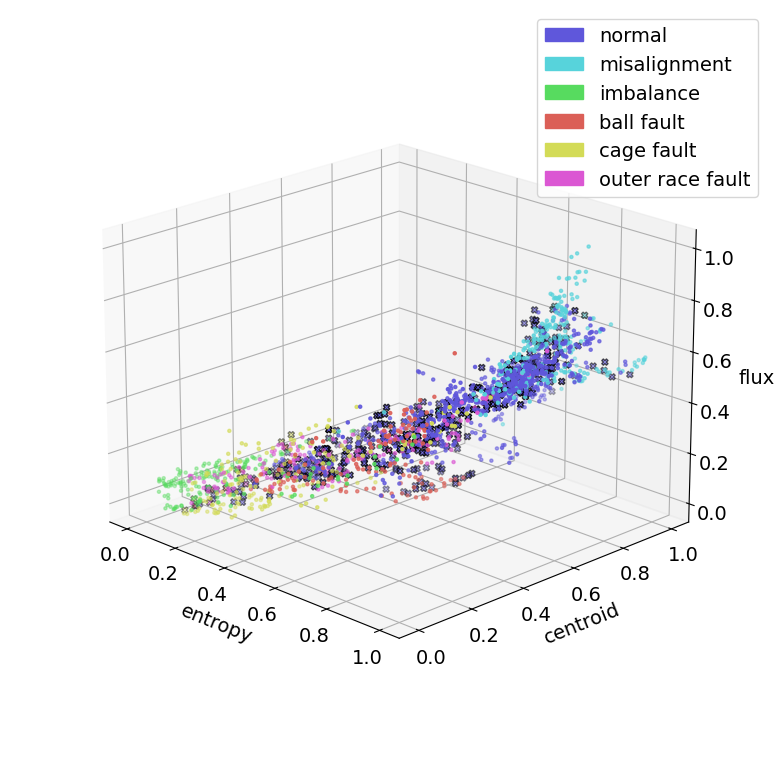
\includegraphics[width=\textwidth]{assets/results/labels/FD-severity.png}
        \caption{Frequency-domain features (severity)}
    \end{subfigure} 
    \caption{3 Best features and their ranges}
\end{figure}
 
%%%%%%%%%%
\clearpage

\subsection{Incremental learning}
% Ordering of severity
\begin{figure}[ht]
    \centering
    \begin{subfigure}[b]{0.3\textwidth}
        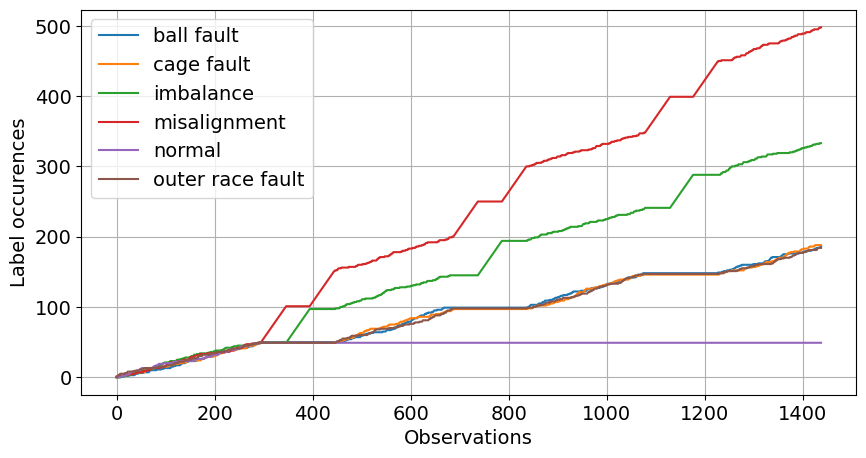
\includegraphics[width=\textwidth]{assets/results/incremental-learning/order-natural.png}
        \caption{Order by raising severity}
    \end{subfigure}
    \hfill
    \begin{subfigure}[b]{0.3\textwidth}
        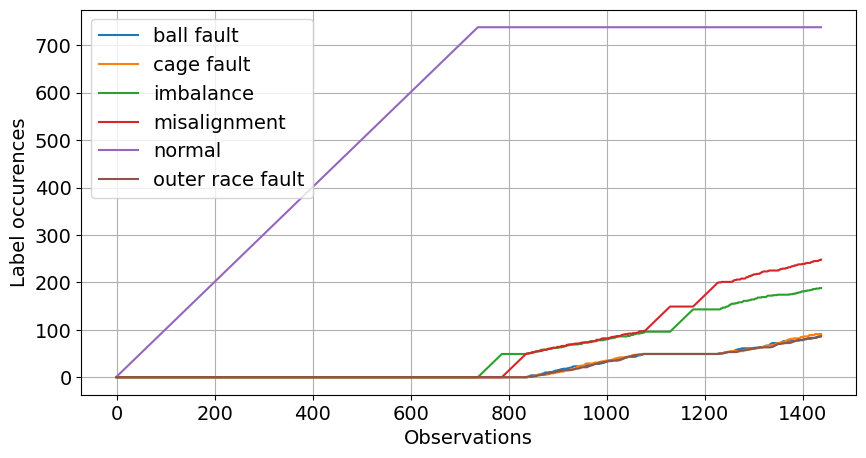
\includegraphics[width=\textwidth]{assets/results/incremental-learning/order-severity.png}
        \caption{Order after relabeing normal class}
    \end{subfigure}
    \hfill
    \begin{subfigure}[b]{0.3\textwidth}
        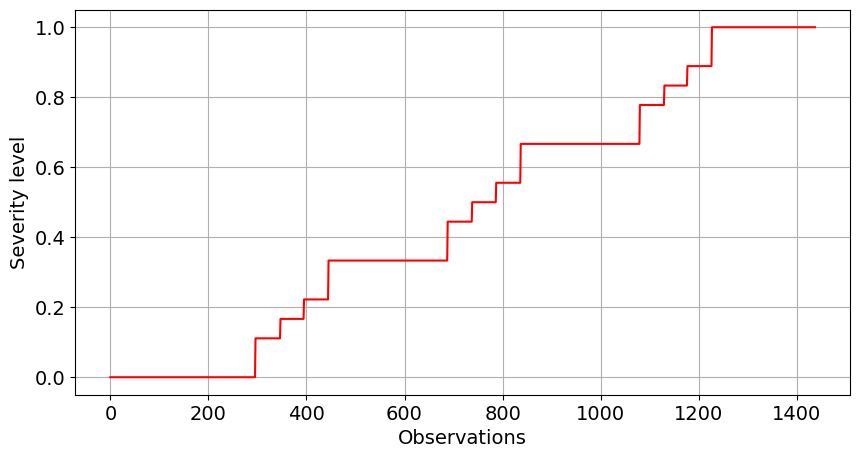
\includegraphics[width=\textwidth]{assets/results/incremental-learning/severity-levels.png}
        \caption{Order of relative severity levels}
    \end{subfigure}
    \caption{Ordering of faults}
\end{figure}


% Tumbling windows
\begin{figure}[h]
    \centering
    \begin{subfigure}[b]{0.48\textwidth}
        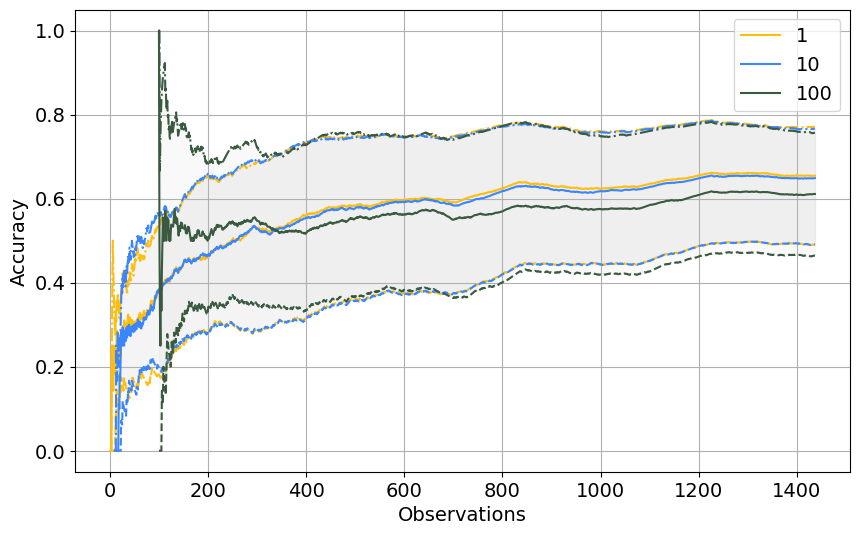
\includegraphics[width=\textwidth]{assets/results/incremental-learning/tumbling-TD.png}
        \caption{Time-domain features}
    \end{subfigure}
    \hfill
    \begin{subfigure}[b]{0.48\textwidth}
        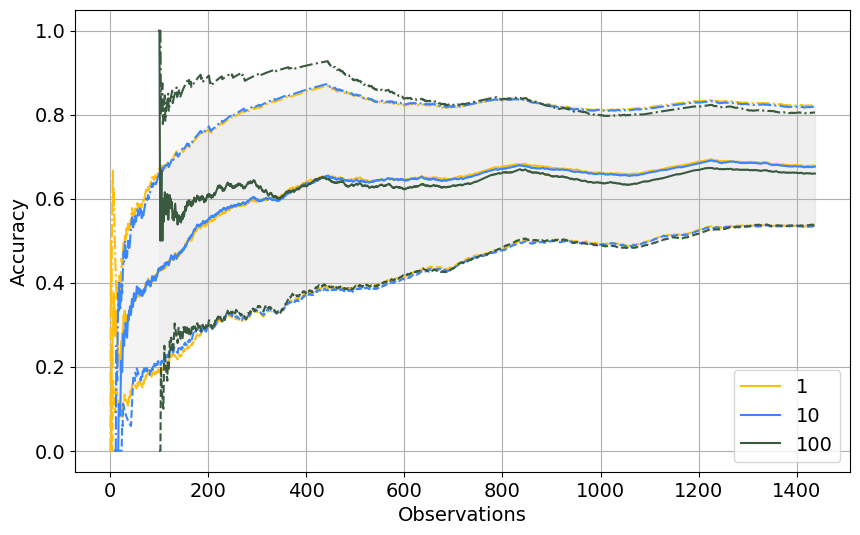
\includegraphics[width=\textwidth]{assets/results/incremental-learning/tumbling-FD.png}
        \caption{Frequency-domain features}
    \end{subfigure}
    \hfill
    \begin{subfigure}[b]{0.48\textwidth}
        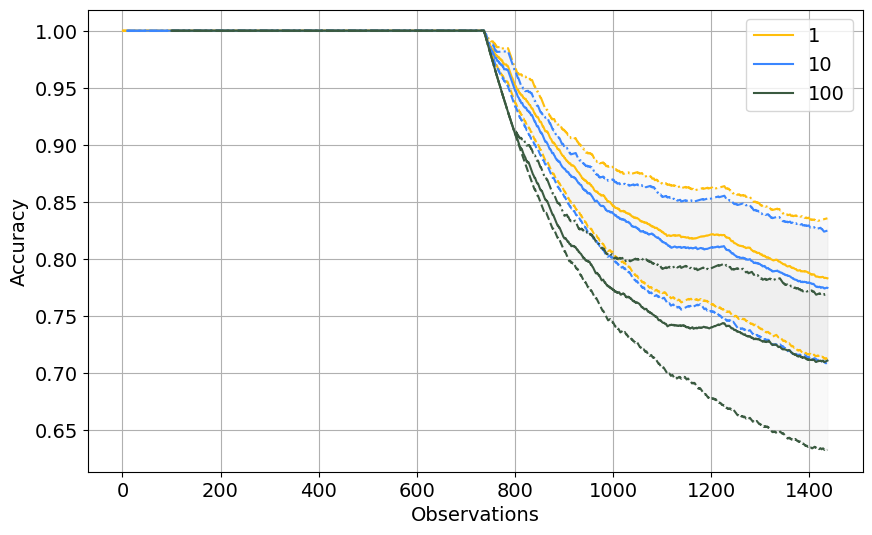
\includegraphics[width=\textwidth]{assets/results/incremental-learning/tumbling-TD-severity.png}
        \caption{Time-domain features (severity)}
    \end{subfigure}
    \hfill
    \begin{subfigure}[b]{0.48\textwidth}
        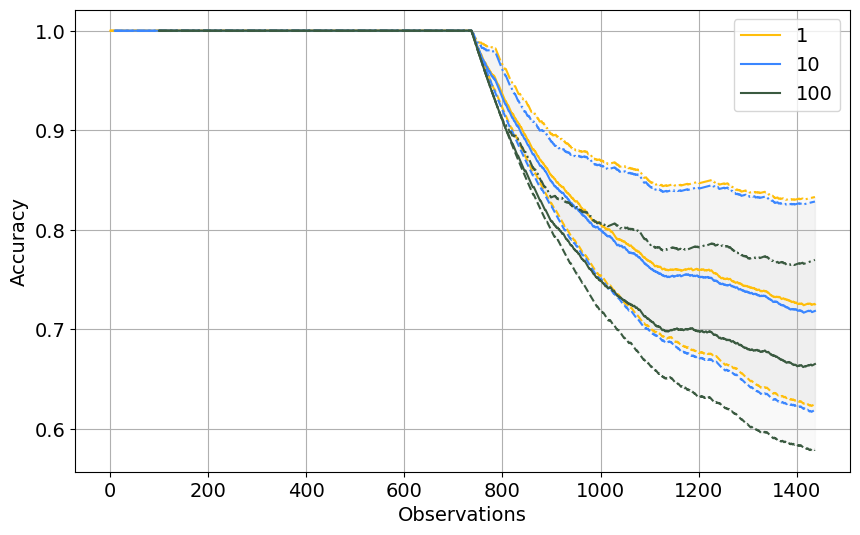
\includegraphics[width=\textwidth]{assets/results/incremental-learning/tumbling-FD-severity.png}
        \caption{Frequency-domain features (severity)}
    \end{subfigure} 
    \caption{Tumbling window in incremental learning}
\end{figure}


% % Label skips and parts of dataset
\begin{figure}[h]
    \centering
    \begin{subfigure}[b]{0.48\textwidth}
        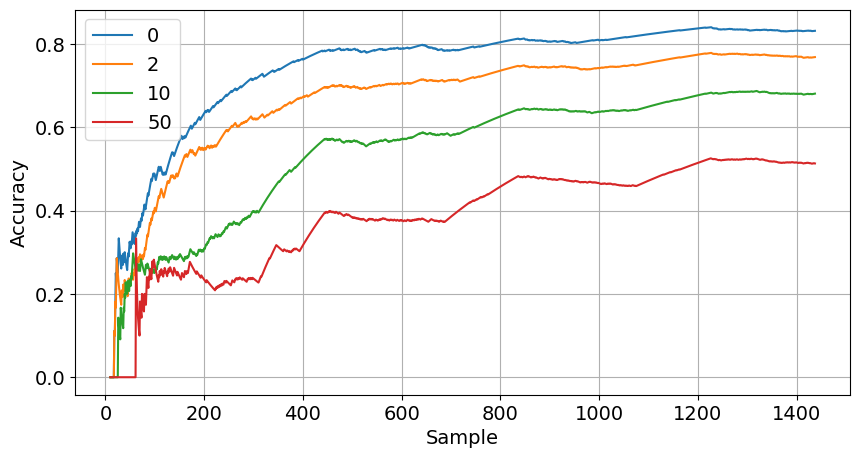
\includegraphics[width=\textwidth]{assets/results/incremental-learning/all-features-TD-skip.png}
        \caption{Time-domain features}
    \end{subfigure}
    \hfill
    \begin{subfigure}[b]{0.48\textwidth}
        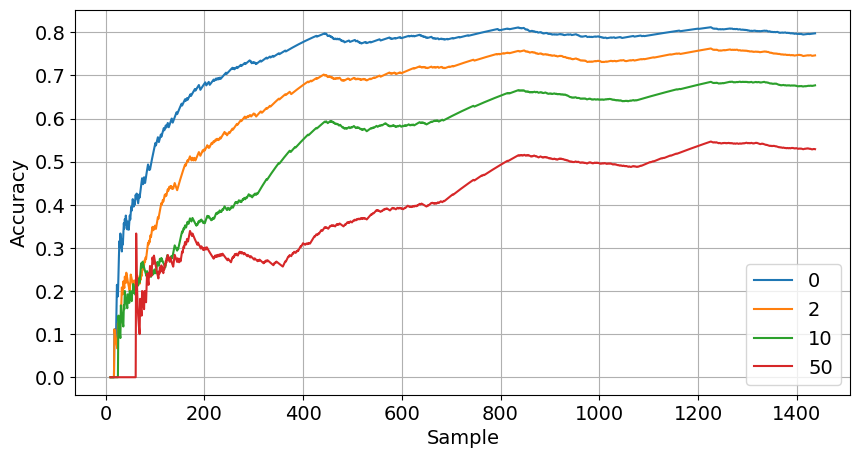
\includegraphics[width=\textwidth]{assets/results/incremental-learning/all-features-FD-skip.png}
        \caption{Frequency-domain features}
    \end{subfigure}
    \hfill
    \begin{subfigure}[b]{0.48\textwidth}
        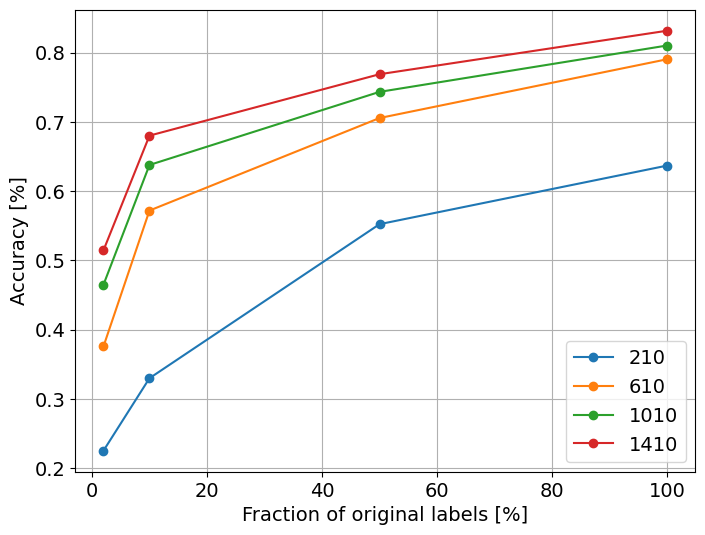
\includegraphics[width=\textwidth]{assets/results/incremental-learning/skip-labels-TD.png}
        \caption{Time-domain features}
    \end{subfigure}
    \hfill
    \begin{subfigure}[b]{0.48\textwidth}
        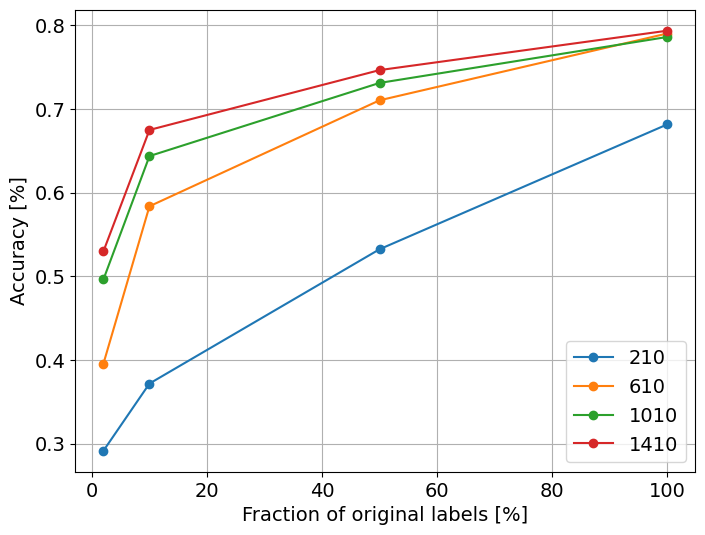
\includegraphics[width=\textwidth]{assets/results/incremental-learning/skip-labels-FD.png}
        \caption{Frequency-domain features}
    \end{subfigure} 
    \caption{Skip labels in incremental learning}
\end{figure}


\begin{figure}[h]
    \centering
    \begin{subfigure}[b]{0.48\textwidth}
        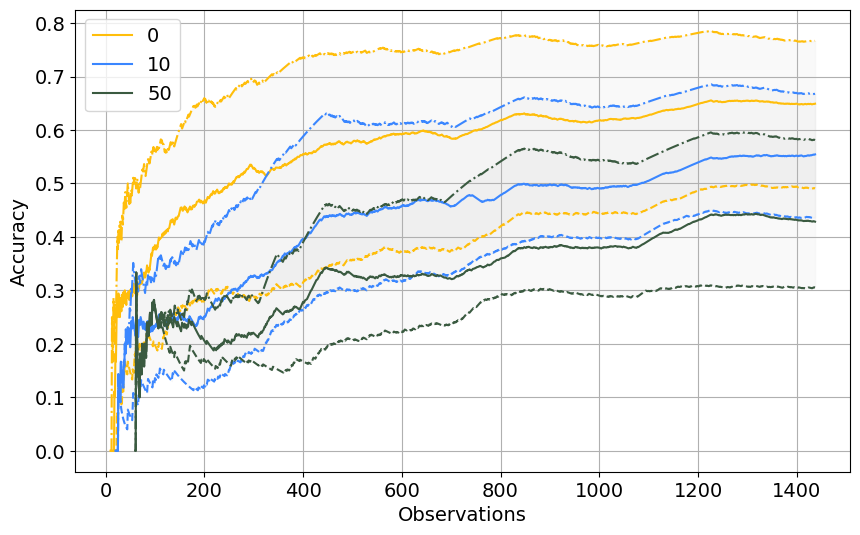
\includegraphics[width=\textwidth]{assets/results/incremental-learning/skip-label-TD.png}
        \caption{Time-domain features}
    \end{subfigure}
    \hfill
    \begin{subfigure}[b]{0.48\textwidth}
        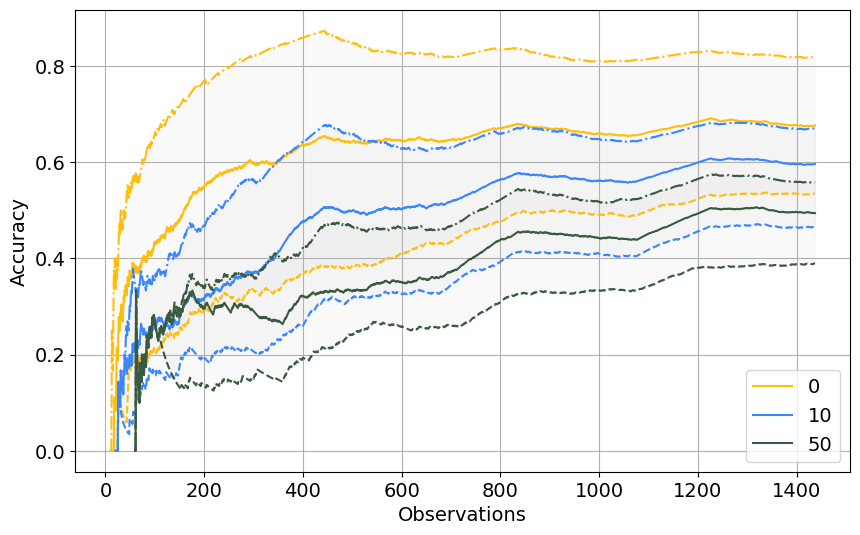
\includegraphics[width=\textwidth]{assets/results/incremental-learning/skip-label-FD.png}
        \caption{Frequency-domain features}
    \end{subfigure}
    \hfill
    \begin{subfigure}[b]{0.48\textwidth}
        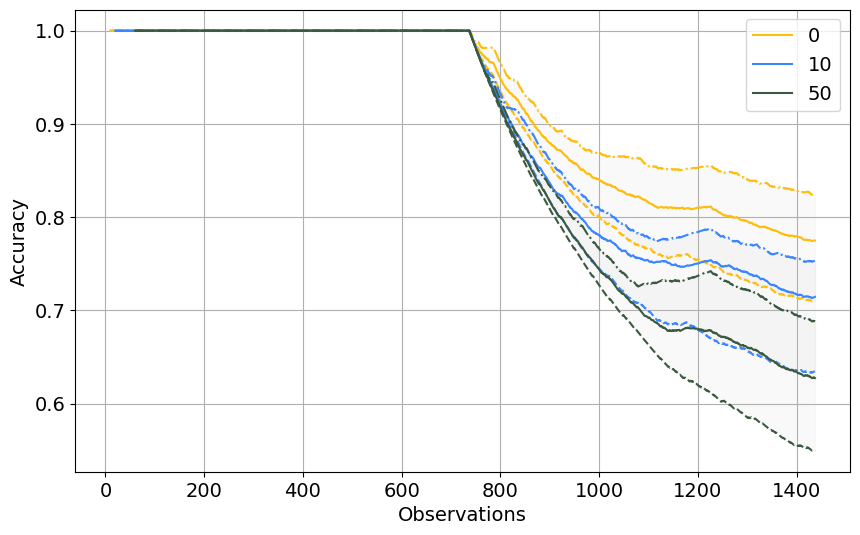
\includegraphics[width=\textwidth]{assets/results/incremental-learning/skip-label-TD-severity.png}
        \caption{Time-domain features (severity)}
    \end{subfigure}
    \hfill
    \begin{subfigure}[b]{0.48\textwidth}
        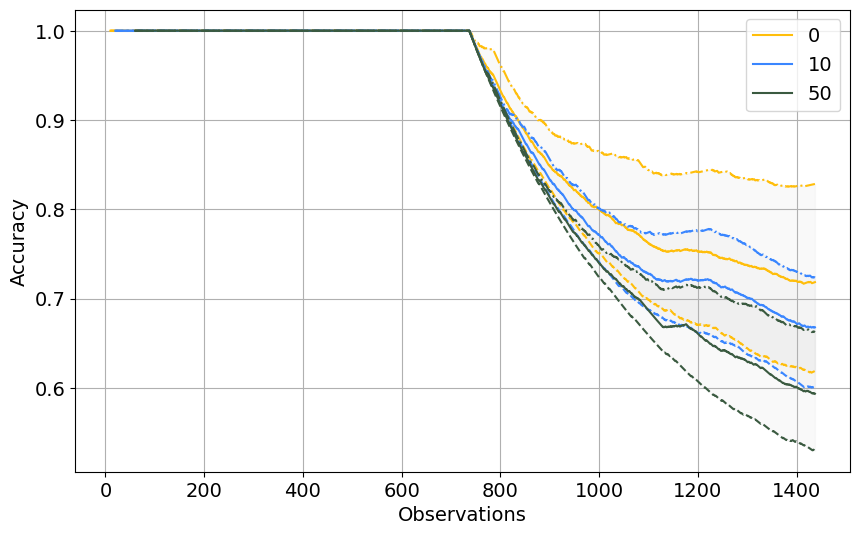
\includegraphics[width=\textwidth]{assets/results/incremental-learning/skip-label-FD-severity.png}
        \caption{Frequency-domain features (severity)}
    \end{subfigure} 
    \caption{Skip labels in incremental learning with different sizes}
\end{figure}



\section{Industrial dataset analysis}

\subsection{Data logger validation}

\begin{figure}[h]
    \centering
    \begin{subfigure}[b]{0.49\textwidth}
        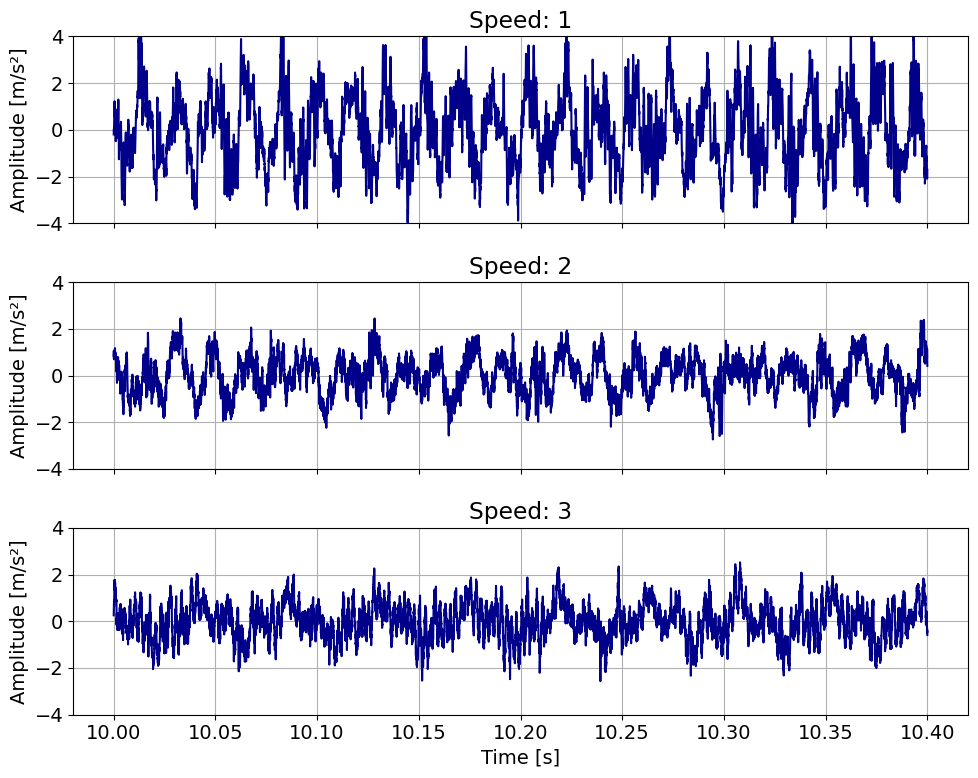
\includegraphics[width=\textwidth]{assets/results/standing-fan/waveform.png}
        \caption{Time waveform}
    \end{subfigure}
    \hfill
    \begin{subfigure}[b]{0.49\textwidth}
        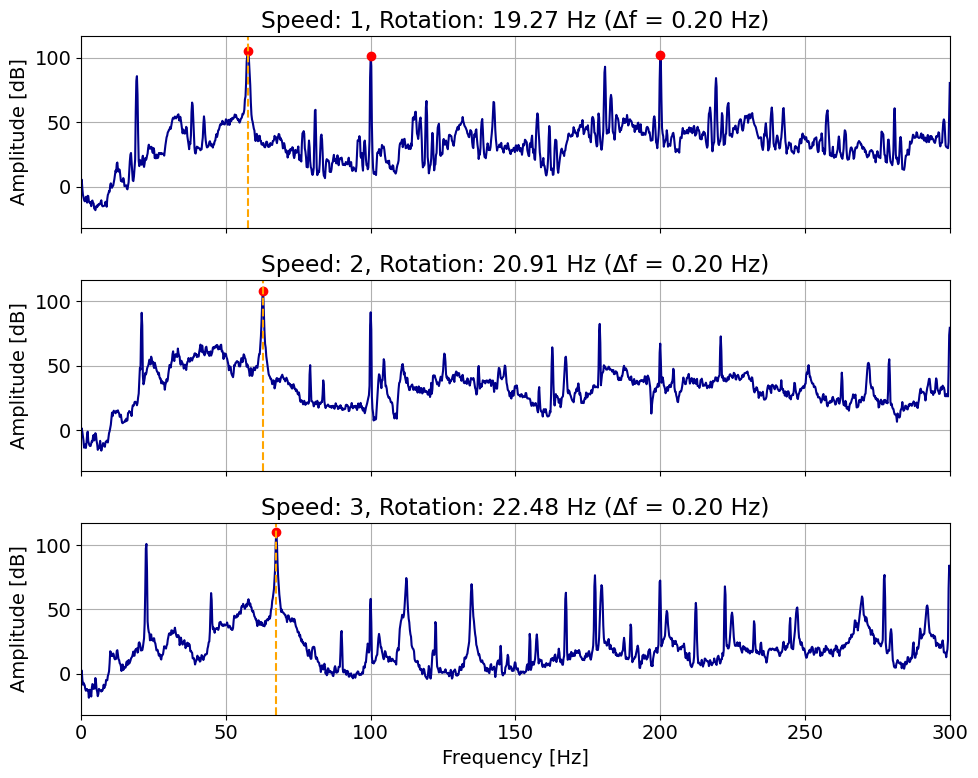
\includegraphics[width=\textwidth]{assets/results/standing-fan/standing-fan-accel.png}
        \caption{Estimation of rotation speed}
    \end{subfigure}
    \caption{Vibrations from the back of a standing fan in radial direction}
\end{figure}


\subsection{Feature ranges}
% Amplitude histograms - 20m/s^2, 40m/s^2, 150m/s^
% Histograms of machinery measurements


% Box plots of features
\begin{figure}[h]
    \centering
    \begin{subfigure}[b]{\textwidth}
        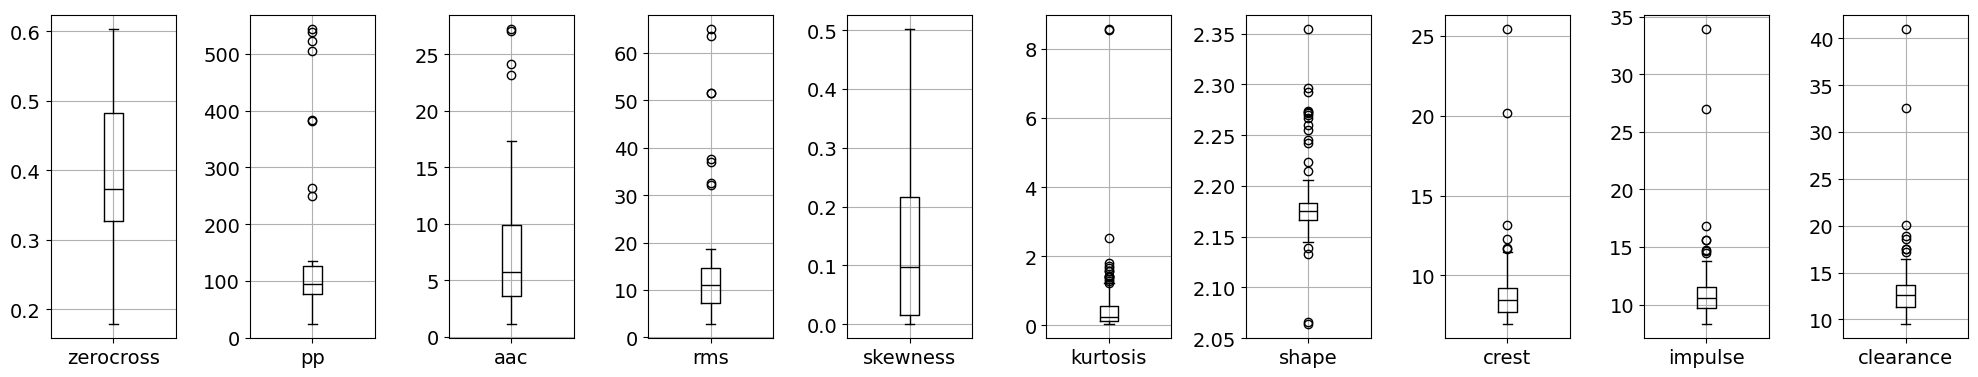
\includegraphics[width=\textwidth]{assets/results/feature-values/pumps-TD-dim-3.png}
        \caption{Time-domain features}
    \end{subfigure}
    \hfill
    \begin{subfigure}[b]{\textwidth}
        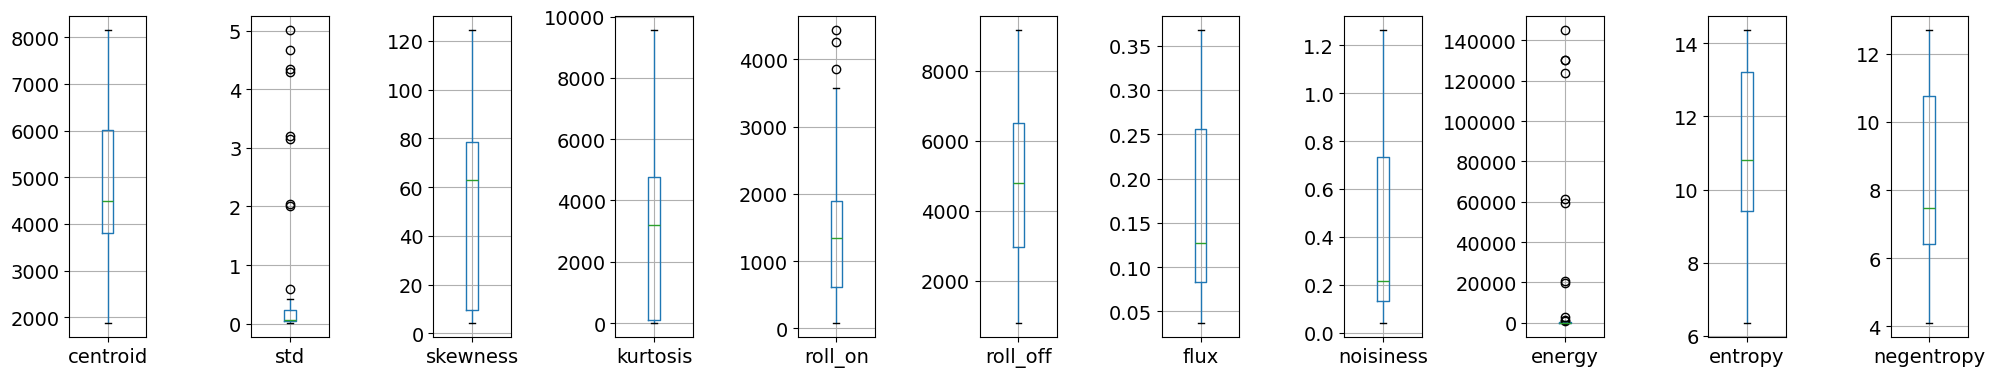
\includegraphics[width=\textwidth]{assets/results/feature-values/pumps-FD-dim-3.png}
        \caption{Frequency-domain features}
    \end{subfigure}
    \caption{Feature range in pumps}
\end{figure}

\subsection{Time-frequency waveforms}
\begin{figure}[h]
    \centering
    \begin{subfigure}[b]{0.32\textwidth}
        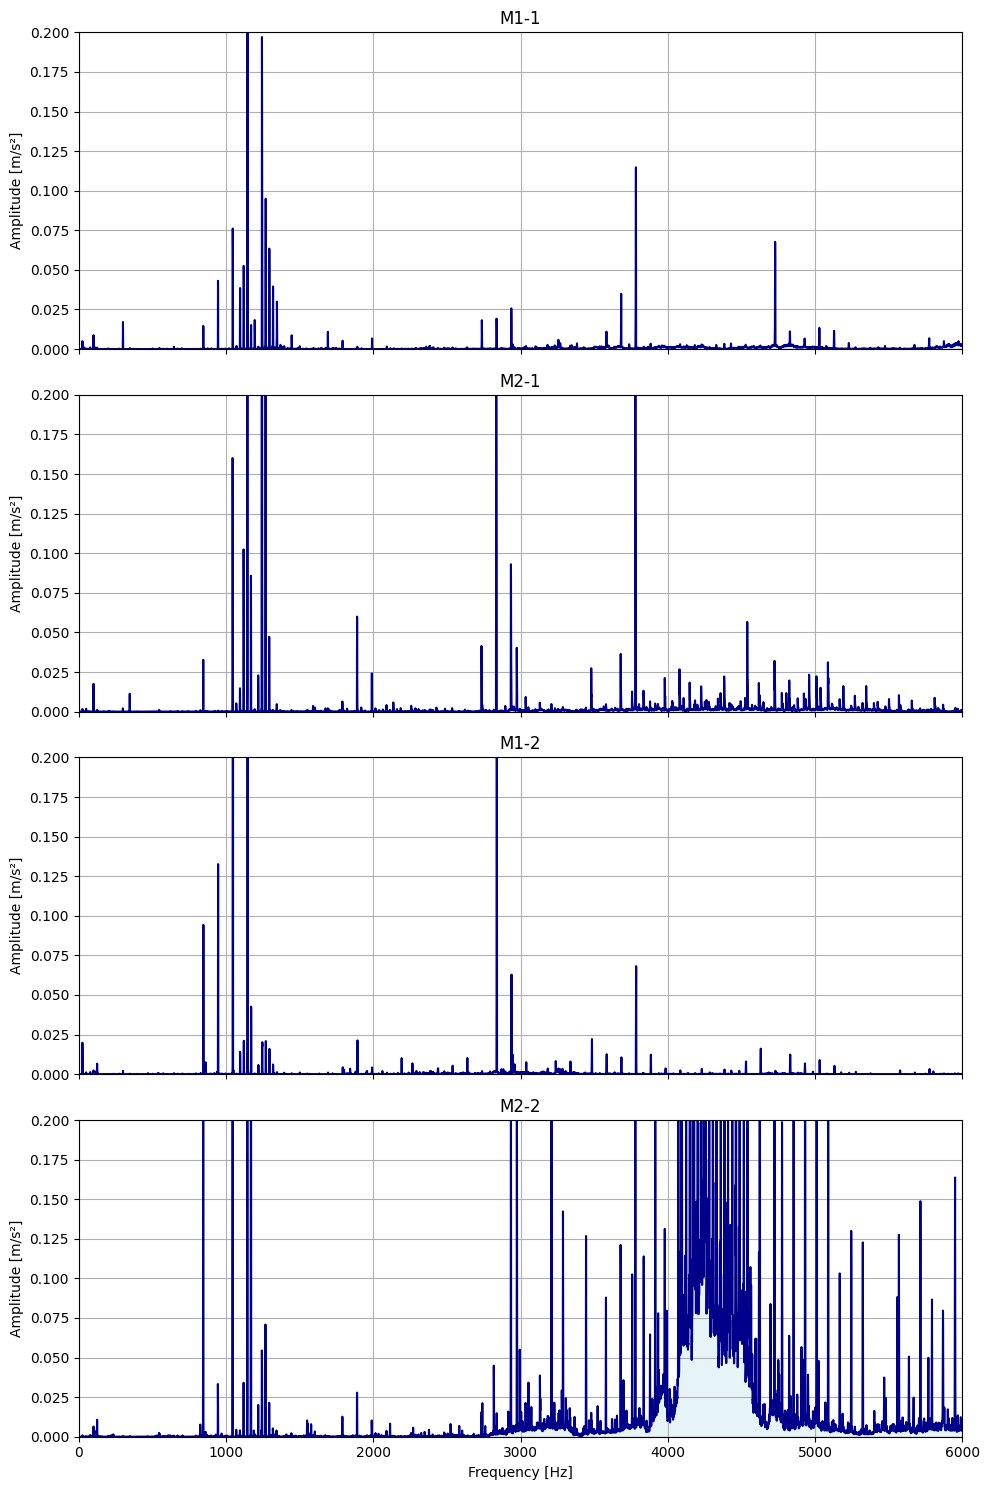
\includegraphics[width=\textwidth]{assets/results/eda/frequency-spectrum-motors.png}
        \caption{Motors}
    \end{subfigure}
    \hfill
    \begin{subfigure}[b]{0.32\textwidth}
        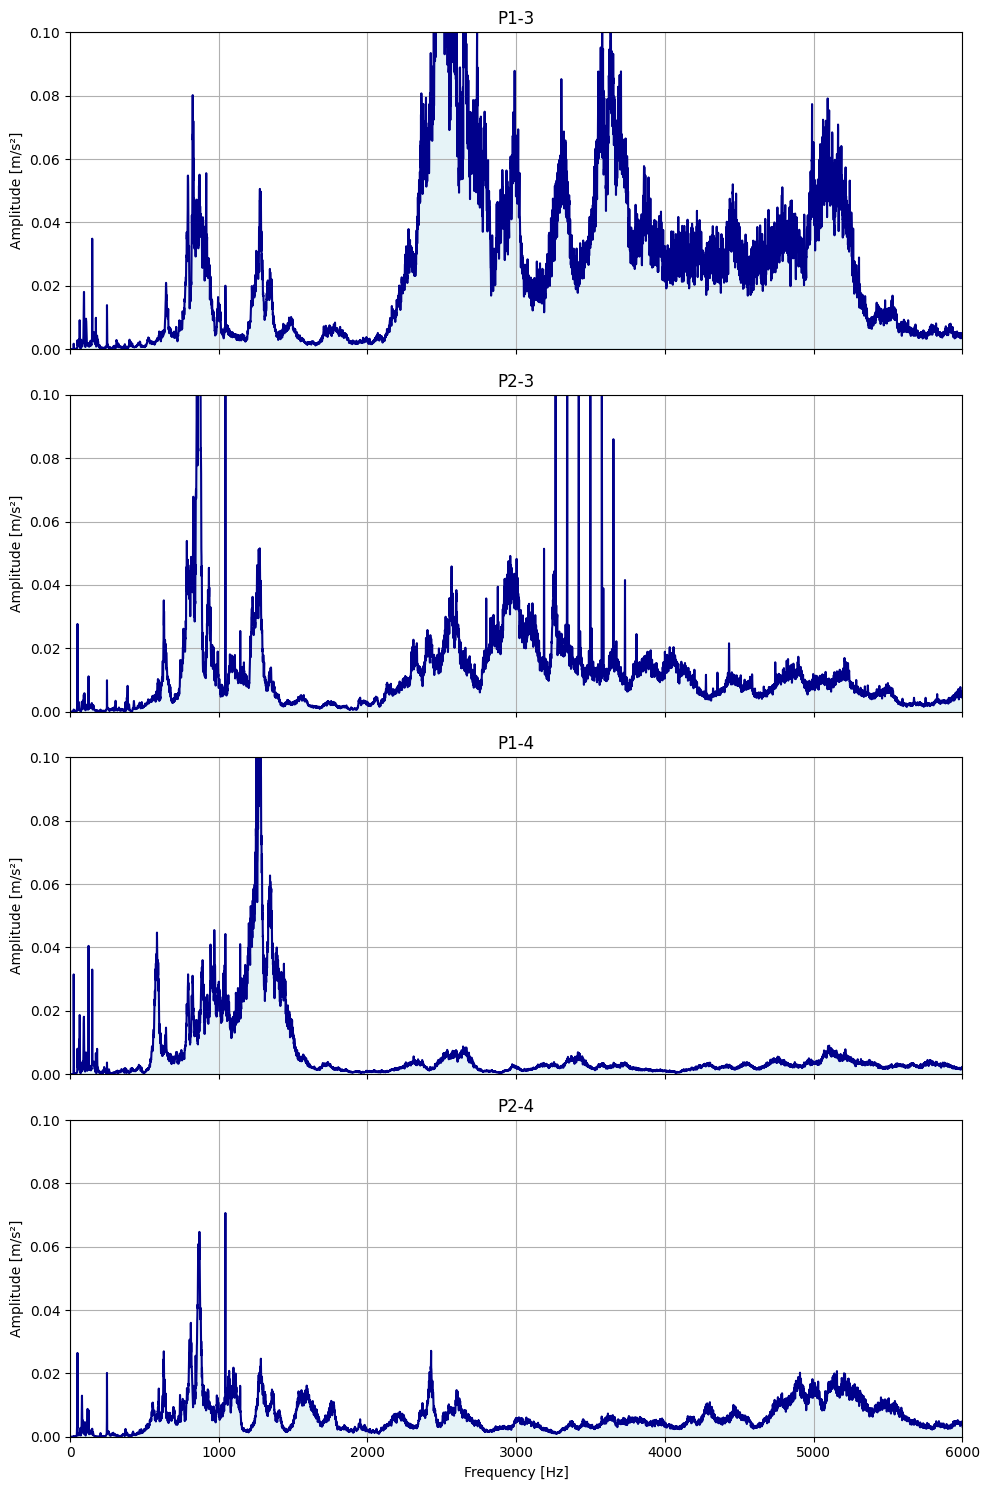
\includegraphics[width=\textwidth]{assets/results/eda/frequency-spectrum-pumps.png}
        \caption{Pumps}
    \end{subfigure}
    \hfill
    \begin{subfigure}[b]{0.32\textwidth}
        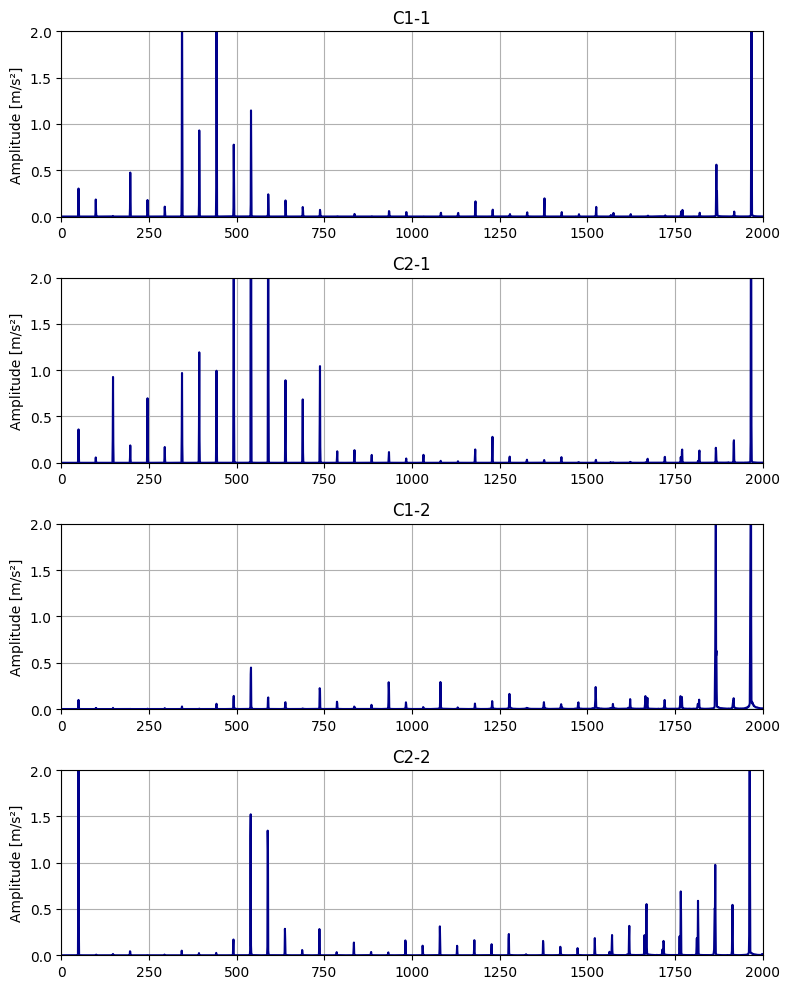
\includegraphics[width=\textwidth]{assets/results/eda/frequency-spectrum-compressors.png}
        \caption{Compressor}
    \end{subfigure} 
    \caption{Frequency domain}
\end{figure}


% Time-frequency spectrum

% Low frequencies (under 1KHz)

\begin{figure}[h]
    \centering
    \begin{subfigure}[b]{0.48\textwidth}
        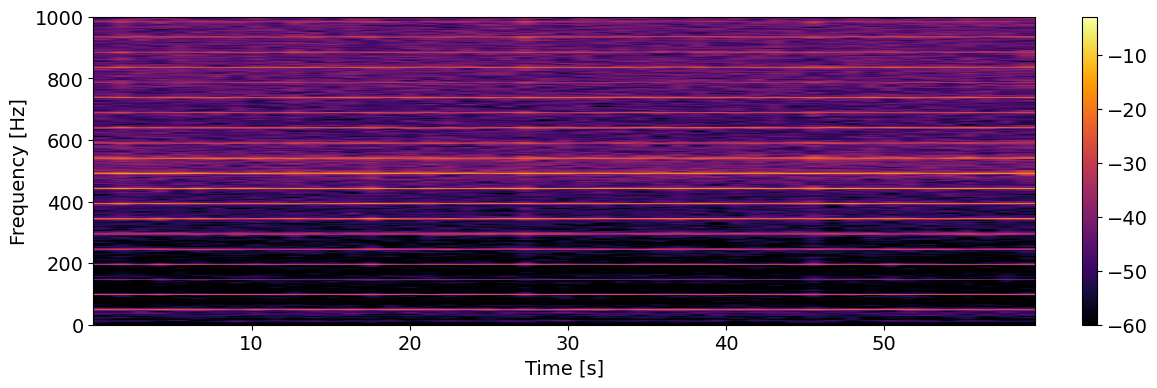
\includegraphics[width=\textwidth]{assets/results/time-frequency-spectrum/K3-z-STFT-1kHz.png}
        \caption{K3}
    \end{subfigure}
    \hfill
    \begin{subfigure}[b]{0.48\textwidth}
        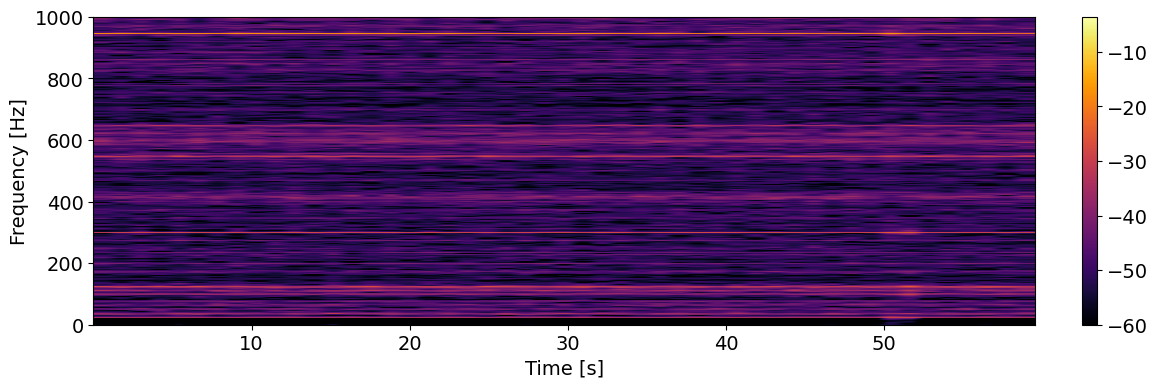
\includegraphics[width=\textwidth]{assets/results/time-frequency-spectrum/M1-2-z-STFT-1kHz.png}
        \caption{M1-2}
    \end{subfigure}
    \hfill
    \begin{subfigure}[b]{0.48\textwidth}
        \includegraphics[width=\textwidth]{assets/results/time-frequency-spectrum/P1-3-z-STFT-1kHz.png}
        \caption{P1-3}
    \end{subfigure}
	\hfill
	\begin{subfigure}[b]{0.48\textwidth}
        \includegraphics[width=\textwidth]{assets/results/time-frequency-spectrum/P3-3-z-STFT-1kHz.png}
        \caption{P3-3}
    \end{subfigure}
    \caption{Time frequency spectrum}
\end{figure}


\begin{figure}[h]
    \centering
    \begin{subfigure}[b]{0.48\textwidth}
        \includegraphics[width=\textwidth]{assets/results/time-frequency-spectrum/P1-slow-down.png}
        \caption{Pump P1 turns off}
    \end{subfigure}
    \hfill
    \begin{subfigure}[b]{0.48\textwidth}
        \includegraphics[width=\textwidth]{assets/results/time-frequency-spectrum/P2-speed-up.png}
        \caption{Pump P2 turn on}
    \end{subfigure}
\end{figure}

\subsection{Bearing defect frequencies}
% Domain expert analysis
% Bearing frequencies table
\begin{table}[h]
\centering
\begin{tabular}{|l|r|r|r|}
\hline
\textbf{Placement}     & \multicolumn{1}{l|}{\textbf{Motor \#1}} & \multicolumn{1}{l|}{\textbf{Motor \#2}} & \multicolumn{1}{l|}{\textbf{Pump \#3 \& \#4}} \\ \hline
\textbf{Bearing}       & \multicolumn{1}{l|}{6319-C3}            & \multicolumn{1}{l|}{6324-C3}            & \multicolumn{1}{l|}{6317-2Z}                  \\ \hline
\textbf{$n$}           & 8                                       & 8                                       & 8                                             \\ \hline
\textbf{$f_s$}         & 1493                                    & 1493                                    & 1493                                          \\ \hline
\textbf{$d$ {[}mm{]}}  & 33.12                                   & 41.28                                   & 30.00                                         \\ \hline
\textbf{$D$ {[}mm{]}}  & 147.5                                   & 190.0                                   & 132.5                                         \\ \hline
\textbf{$\beta$}       & 0                                       & 0                                       & 0                                             \\ \hline
\textbf{RPM {[}Hz{]}}  & 24.88                                   & 24.88                                   & 24.88                                         \\ \hline
\textbf{BPFO {[}Hz{]}} & 77.18                                   & 77.91                                   & 77.00                                         \\ \hline
\textbf{BPFI {[}Hz{]}} & 121.88                                  & 121.16                                  & 122.07                                        \\ \hline
\textbf{BSF {[}Hz{]}}  & 58.20                                   & 59.97                                   & 57.77                                         \\ \hline
\textbf{FTF {[}Hz{]}}  & 9.65                                    & 9.74                                    & 9.63                                          \\ \hline
\end{tabular}
\end{table}

% Bearing defect frequencies
\begin{figure}[h]
    \centering
    \begin{subfigure}[b]{0.24\textwidth}
        \includegraphics[width=\textwidth]{assets/results/defects/motors.png}
        \caption{Motors}
    \end{subfigure}
    \hfill
    \begin{subfigure}[b]{0.24\textwidth}
        \includegraphics[width=\textwidth]{assets/results/defects/motors-dB.png}
        \caption{Pumps}
    \end{subfigure}
    \begin{subfigure}[b]{0.24\textwidth}
        \includegraphics[width=\textwidth]{assets/results/defects/pumps.png}
        \caption{Motors}
    \end{subfigure}
    \hfill
    \begin{subfigure}[b]{0.24\textwidth}
        \includegraphics[width=\textwidth]{assets/results/defects/pumps-dB.png}
        \caption{Pumps dB}
    \end{subfigure}
\end{figure}


\subsection{Pump long-term monitoring}

% Total vibration levels - challange - long-live span (5 years)
\begin{figure}[h]
    \centering
    \begin{subfigure}[b]{0.49\textwidth}
        \includegraphics[width=\textwidth]{assets/results/ksb-cloud/p1.png}
        \caption{Pump P1}
    \end{subfigure}
    \hfill
    \begin{subfigure}[b]{0.49\textwidth}
        \includegraphics[width=\textwidth]{assets/results/ksb-cloud/p2.png}
        \caption{Pump P2}
    \end{subfigure}
    \caption{Vibration levels}
\end{figure}

% Reverse engineer of spectra (low resolution)
\begin{figure}[h]
    \centering
    \includegraphics[width=0.8\textwidth]{assets/results/ksb-cloud/spectrum.png}
    \caption{Frequency spectrum}
\end{figure}


